 % =============================================================================
% Real-Time Intelligence and Scalable Architecture for Robotics
% Springer (svjour3) formatted version (CIS target)
% =============================================================================
\RequirePackage{fix-cm}
\documentclass[smallextended]{svjour3}
\smartqed  % flush right qed marks, e.g. at end of proof

\journalname{Complex \& Intelligent Systems}

\usepackage[numbers,sort&compress]{natbib}
\usepackage{amsmath,amssymb,amsfonts}
\usepackage[final]{microtype}
\usepackage{graphicx}
\usepackage{textcomp}
\usepackage[table]{xcolor}
\usepackage{colortbl}
\usepackage{booktabs}
\usepackage{array}
\usepackage{enumitem}
\usepackage{needspace} % prevent orphan section headings at page bottom
\usepackage[hidelinks]{hyperref}
\usepackage{caption}
\usepackage{placeins}
\usepackage{subcaption}
\usepackage{fancyvrb} % better verbatim blocks (breaklines/fontsize)

\usepackage{calc}
\usepackage{ifthen}

\usepackage{tikz}
\usetikzlibrary{positioning,arrows.meta,fit,shapes.geometric,calc,backgrounds,bending}

% Reduce overfull boxes without changing meaning.
\emergencystretch=2em

%% Table helpers
\newcolumntype{L}[1]{>{\raggedright\arraybackslash}p{#1}}
\newcolumntype{C}[1]{>{\centering\arraybackslash}p{#1}}
\definecolor{tablehead}{HTML}{2E75B6}
\definecolor{tablealt}{HTML}{F2F7FC}

%% Simple callout environment (IEEE-friendly)
\newenvironment{designbox}[1]{%
  \begin{quote}\small\noindent\textbf{#1}\par\smallskip%
}{\end{quote}}

% =============================================================================
% Experiment setup macros (kept in a separate file for consistency)
% =============================================================================
% =============================================================================
% Illustrative experiment binding (reference-design paper; no hardware run).
% Replace entire definitions when you have measured results. Do not present
% these strings as empirical findings from a completed campaign.
% =============================================================================
\providecommand{\PilotBindingScope}{%
This binding is \emph{illustrative}: it fixes notation, units, and reporting slots for a future pilot. It is not a claim that the experiments below were executed on this stack.}

\providecommand{\PilotPlatformCPU}{%
Example: NVIDIA Jetson Orin NX module, 8$\times$ Cortex-A78AE (illustrative nominal 2.0\,GHz cap).}
\providecommand{\PilotPlatformGPU}{%
Example: integrated Ampere-class GPU with configurable power/clock caps (vendor max-power mode off for repeatability).}
\providecommand{\PilotPlatformRAM}{%
Example: 16\,GiB LPDDR5 (single-channel configuration as shipped on the module).}
\providecommand{\PilotOSKernel}{%
Example: Ubuntu 22.04 LTS with a generic 5.15.x LTS kernel and unattended upgrades disabled during data collection (recommended).}
\providecommand{\PilotPowerMode}{%
Example: \textsc{nvpmodel} maximum-performance profile for the module class (document exact ID used).}
\providecommand{\PilotGovernor}{%
Example: \texttt{schedutil} on CPU clusters; GPU clocks left at vendor defaults unless pinned explicitly.}

\providecommand{\PilotROS}{%
Example: ROS~2 Humble Hawksbill.}
\providecommand{\PilotExecutor}{%
Example: \texttt{rclcpp} multithreaded executor; perception callbacks in one mutually exclusive group, monitor/supervisor in another to reduce self-interference.}
\providecommand{\PilotDDS}{%
Example: Fast DDS with vendor defaults unless a latency study fixes discovery and transport settings.}
\providecommand{\PilotQoSCamera}{%
Example: \texttt{/camera/image\_raw} with \texttt{sensor\_data} QoS profile (best effort, depth\,1, keep last) unless the sensor driver requires reliable delivery.}
\providecommand{\PilotQoSDetections}{%
Example: \texttt{/detections} with reliable delivery, depth\,1, keep last, same clock domain as upstream image.}

\providecommand{\PilotLatencyStart}{%
\texttt{sensor\_msgs/Image.header.stamp} on ingress to the perception node (or driver publish time if that is your ground truth).}
\providecommand{\PilotLatencyEnd}{%
Wall time when the node publishes \texttt{vision\_msgs/Detection2DArray} (or your project's equivalent detections message).}
\providecommand{\PilotLatencyClock}{%
ROS clock on both endpoints (\texttt{rclcpp::ClockType::ROS\_TIME}) with verified time synchronization if any component uses a different domain.}

\providecommand{\PilotDeadlineMs}{%
$D=33$\,ms (illustrative 30\,Hz perception budget; replace with contract value from your TIC).}
\providecommand{\PilotMissCounting}{%
One miss is counted per completed frame whose measured camera$\rightarrow$detections latency exceeds $D$ (per-frame accounting; burst statistics optional).}
\providecommand{\PilotWeaklyHard}{%
Weakly-hard $(m,k)$ not used in this illustrative binding (enable only if your TIC states an $(m,k)$ window over misses).}

\providecommand{\PilotStressors}{%
Example pattern: \texttt{stress-ng --cpu 4 --cpu-method matrixprod} during the stress segment only; optional GPU contention via a second CUDA workload with fixed kernel duration (document both).}
\providecommand{\PilotAffinity}{%
Example: pin perception and monitor nodes to CPUs 0--3; pin stressor to CPUs 4--7 on an 8-core module (or document ``no pinning'' if left default).}
\providecommand{\PilotProtocolDurations}{%
Example segment lengths matching common pilot guidance: nominal 7.5\,min, induced load 7.5\,min, recovery 5\,min (20\,min total per repetition).}

\providecommand{\PilotRuns}{%
Measured runs: $N=0$ in this manuscript draft. For acceptance-grade reporting, plan $N\ge 5$ independent repetitions with cold/warm start policy fixed.}
\providecommand{\PilotCIApproach}{%
Planned: 95\% bootstrap confidence intervals on \emph{run-level} summaries (e.g., run mean miss rate, run p95 latency) once $N$ traces exist; scripts under \texttt{scripts/} provide a CSV template and \texttt{generate\_miss\_rate\_ci\_figure.py}.}

\providecommand{\PilotCAAIClaims}{%
Expected qualitative signatures to verify when measured: (i) lower miss rate than fixed Tier~1 under the same stressor because tier-down occurs before repeated deadline violations; (ii) lower tail latency than reactive-after-miss because downgrades precede misses; (iii) envelope mode traces that move with tier and never lag safety-critical deadlines by construction.}
\providecommand{\PilotSensitivityParams}{%
Planned sweeps (example ranges): latency margin threshold 6--12\,ms; supervisor dwell time 50--300\,ms; drift score threshold 0.01--0.05 (replace with your monitor's actual scalars).}
\providecommand{\PilotSensitivityOutcome}{%
Report stability versus those knobs: tier switches per minute, oscillation count, and worst-case consecutive downgrade/upgrade bursts (template plot: \texttt{fig\_pilot\_sensitivity.png}).}

\providecommand{\PilotTierTraceNote}{%
The tier trace in Figure~\ref{fig:tiertrace} may use a compressed second axis for layout; for measured work, regenerate from tier logs with \texttt{generate\_tier\_trace.py} using \texttt{--plot-unit min} and \texttt{--phase-ends-sec} aligned to the nominal/stress/recovery segment boundaries.}


\title{Real-Time Intelligence and Scalable Architecture for Robotics}

\author{Sanjay Mishra \and Divya Chukkapalli \and Ganesh R. Naik}

\institute{
S. Mishra \at Independent Researcher, Raleigh, NC, USA \\
\email{sanmish4@icloud.com}
\and
D. Chukkapalli \at Independent Researcher, Apex, NC, USA \\
\email{divya.95j@gmail.com}
\and
G. R. Naik \at Torrens University Australia, Adelaide, SA, Australia \\
\email{ganesh.naik@torrens.edu.au}
}

\date{Received: date / Accepted: date}
% The correct dates will be entered by the editor

\titlerunning{Real-Time Intelligence and Scalable Architecture for Robotics}
\authorrunning{Mishra et al.}

\begin{document}

\begin{abstract}
Timing is not a performance metric in robotics; it is a requirement for correctness. This paper is a \textbf{survey/tutorial} with a \textbf{reference-specification} contribution: it treats real-time intelligence and scalable architecture as a single end-to-end systems problem spanning deadlines, execution-time variability, middleware quality of service (QoS), and the edge-cloud division of computation.

Two reference artifacts are specified: the \textbf{Temporal Intelligence Contract (TIC)} and \textbf{Contract-Aware Adaptive Inference (CAAI)}. TIC unifies latency envelopes, uncertainty/drift envelopes, safety fallback behavior, observability requirements, and scalability limits into a machine-readable contract intended for runtime monitoring and auditing. CAAI is a deterministic supervisor specification that consumes TIC-relevant signals (latency margin, calibrated uncertainty, and drift indicators) to switch between perception tiers and to couple tier selection to a corresponding safety envelope.

To support reproducible adoption, the paper provides a minimal contract schema, a conformance checklist, and reporting templates for prototype implementation and measurement. The goal is to make timing and learning-related assumptions explicit and auditable in learning-enabled robotic systems.
\keywords{Real-time robotics \and ROS~2 (Robot Operating System~2) \and robotics middleware \and DDS/QoS \and end-to-end latency monitoring \and edge robotics (edge computing) \and distributed robotic systems \and digital twins for robotics \and machine learning inference deployment \and scalability}
\end{abstract}
\maketitle

% =============================================================================
\section{Introduction}
\label{sec:intro}
Physical processes do not wait for computation. Cars keep moving, actuators keep applying force, environments keep changing, and the software must determine the next action through all of it. In any system coupled to the physical world, timeliness is part of correctness: a right choice that arrives after its deadline is, for the system, the same as a wrong one. A braking scenario makes this concrete. Under typical conditions, the perception-reaction-actuation chain must complete within a narrow window from the moment a driver spots a child stepping into the road. Stretch that chain by even a few seconds, and the outcome changes, the driver did not choose differently, the window for action had simply closed.

Real-time intelligence is the field that takes this constraint seriously, and this is why architecture is as important as algorithmic capability.

The increase in speed of control loops, combined with more complex decision-making and perception pipelines makes the problem more pronounced in robotics. A robot has to perform tasks with deadlines set by mechanics, human proximity, and task-specific contracts, but the software stacks that implement those tasks are now expected to scale from a single prototype to heterogeneous fleets. The scaling of team size, geography, and lifecycle implies new coordination and observability demands, which may subtly compromise timing guarantees unless they are explicitly built in.

\medskip
\noindent\textbf{Roadmap:}\quad
This paper is a \emph{survey/tutorial} with a \emph{reference-specification} contribution: it synthesizes prior work, specifies contract artifacts and switching policies, and provides a prototype decomposition and pilot-experiment template (Section~\ref{sec:eval}) intended to support reproducible evaluation in ROS~2-style systems.
\textit{Unless explicitly stated otherwise, all numerical values in Tables~1, 4, 5, 8, and~9 are synthetic illustrations of reporting format, not measurements from a physical deployment.}

It starts with a literature-based perspective of how real-time constraints and robot software architectures have developed together (Section~\ref{sec:lit}), followed by making these constraints explicit through timing models, schedulability arguments, and worst-case reasoning (Section~\ref{sec:rt}). Section~\ref{sec:scale} then treats scalability as a set of engineering decisions, examining how decomposition, middleware, and the edge-cloud continuum either preserve or violate end-to-end latency guarantees.

Section~\ref{sec:learn} revisits learning from an operational perspective, focused less on model novelty and more on what it takes to run learned components inside a time-bounded pipeline, Section~\ref{sec:cross} covers safety, security, and energy as constraints that feed back into timing rather than as independent nonfunctional concerns. Section~\ref{sec:cases} presents deployed architectural patterns, Section~\ref{sec:contributions} distinguishes this paper's contributions, and Sections~\ref{sec:future} and~\ref{sec:conc} close with open problems and conclusions.

% =============================================================================
\section{Literature Background and Conceptual Foundations}
\label{sec:lit}

\subsection{Survey methodology (scope and selection)}
\label{subsec:survey_method}
This article is written as a survey/tutorial with a reference-specification contribution.
We focused on peer-reviewed literature and widely used engineering documentation across
real-time systems, robotics middleware (ROS/ROS~2 and DDS), edge/cloud robotics, and
learning-enabled autonomy. Sources were identified via keyword search and
backward/forward citation chasing around core terms including \emph{real-time robotics},
\emph{WCET}, \emph{tail latency}, \emph{ROS~2 executor}, \emph{DDS QoS}, \emph{runtime verification},
\emph{uncertainty calibration}, and \emph{distributional drift}. We preferentially included
papers that (i) report end-to-end latency behavior (including variance/tails), (ii) expose
implementation-level factors (executors, scheduling, memory/IPC), or (iii) propose assurance
mechanisms applicable to deployed systems (contracts, monitors, shields). Because the field
evolves quickly, we also cite recent surveys and system reports where they provide an
integrative view or standardized terminology.

\subsection{Real-Time Computing and Control}

The real-time systems community has developed a rich vocabulary for reasoning about when computation must finish, not just how fast it runs on average. This builds on classic work in schedulability, priority assignment, and worst-case execution time (WCET). Textbooks in that area distinguish hard deadlines, where a miss is catastrophic, from soft deadlines, where a miss only degrades quality~\cite{buttazzo2011,liu2000}.
Robotics inherit this distinction in a straightforward way. Emergency braking is a hard deadline problem; missing it can cause direct harm. Keeping a semantic map fresh is generally soft, since a slightly stale map costs efficiency but rarely causes immediate danger.

A long-standing tension emerges when these timing concepts meet the assumptions of control. Classical control theory assumes periodic sampling because it makes stability analysis tractable. Real robot software does not behave that way: it is event-driven, irregular, and its workload shifts from one moment to the next, making timing analysis considerably harder~\cite{buttazzo2011,miskowicz2015}. Event-based control paradigms (e.g.,~\cite{arzen1999}) emerged in part to relax periodic-sampling assumptions. The gap has widened as learned components moved into perception and prediction pipelines. For instance, transformer-based perception models can have input-dependent attention costs and contend with control threads for shared GPU and memory bandwidth.
Weakly hard constraints, which tolerate a bounded number of deadlines missed inside a sliding window, have re-emerged as a practical model for learned pipelines whose per-input runtime cannot be pinned down~\cite{bernat2001}.

\subsection{Middleware and Communication-Centric Design}

Communication became a core architectural concern the moment robot systems grew beyond a single process. The Robot Operating System (ROS) made it standard practice to structure robot software as a graph of loosely coupled nodes exchanging messages, backed by a tooling ecosystem that made integration and reuse practical~\cite{quigley2009}.
ROS~1 was not designed around deterministic timing, so latency variance had to be managed through careful deployment practice rather than through the framework itself. ROS~2 addressed the timing issue more directly by adopting the Data Distribution Service (DDS) and exposing Quality of Service (QoS) policies that map onto robotic timing and reliability requirements. A single QoS setting can, for example, mark a high-rate sensor stream as best-effort while keeping a command channel reliable~\cite{maruyama2016}. Even so, empirical work shows that tail latency depends not only on network conditions but also on executor design and callback scheduling decisions within the runtime~\cite{kronauer2021,casini2019}.
Achieving predictable behavior requires end-to-end discipline across memory allocation, inter-process communication configuration, and OS kernel setup, with measurements taken to identify exactly where variance enters the system~\cite{ros2realtime2023,ros2executor2024}.

The same end-to-end perspective applies below the middleware layer. In industrial networks, Time-Sensitive Networking (TSN) is often seen as a path to bounded-latency communication, yet measurement studies show that its guarantees can be undermined by integration choices and cross-traffic in real deployments~\cite{wfcs2023tsn}.

Two existing approaches are worth distinguishing from {TIC}. {AUTOSAR} Timing Extensions provide a timing contract model for automotive {ECU} development with runtime monitoring of timing constraints~\cite{autosar2020}. In principle, one could imagine adding ``uncertainty'' and ``drift'' signals to an {AUTOSAR} timing chain, but this would still leave key gaps for learning-enabled robots: (i) {AUTOSAR} timing chains focus on deterministic execution/communication semantics, while learned components require explicit calibration/drift evidence (Section~\ref{sec:tic_schema}); (ii) the standard does not define how probabilistic evidence links to an executable safety-degradation policy; and (iii) robotics stacks commonly span heterogeneous compute (SoC+GPU), middleware (DDS), and edge/cloud paths that sit outside the traditional in-vehicle ECU scope.

{ROSRV} provides runtime verification for {ROS} by monitoring message-level safety properties via formal specifications~\cite{huang2014rosrv}, but operates primarily at the communication protocol/property level and does not treat timing envelopes, uncertainty calibration, drift monitoring, and scalability constraints as a single auditable contract artifact.

Table~\ref{tab:tic_comparison} summarizes the gap: TIC is not ``yet another timing budget format,'' but a cross-layer contract that binds timing to learning-specific evidence and to an explicit fallback state machine.

\begin{table*}[t]
  \centering
  \small
  \setlength{\tabcolsep}{3pt}
  \caption{Clause-level comparison of TIC vs. existing timing/monitoring approaches. ``Native'' means the concept is explicitly modeled and intended for runtime checking; ``Partial'' means it can be approximated with custom signals/properties but is not first-class.}
  \label{tab:tic_comparison}
  \renewcommand{\arraystretch}{1.15}
  \begin{tabular}{@{}L{0.22\linewidth}L{0.14\linewidth}L{0.14\linewidth}L{0.14\linewidth}L{0.14\linewidth}L{0.17\linewidth}@{}}
    \arrayrulecolor{black}\toprule
    \rowcolor{tablehead}
    \textcolor{white}{\textbf{Capability}} &
    \textcolor{white}{\textbf{AUTOSAR TIMEX}} &
    \textcolor{white}{\textbf{ROSRV}} &
    \textcolor{white}{\textbf{ROS\-Monitoring}} &
    \textcolor{white}{\textbf{ROS~2 Lifecycle}} &
    \textcolor{white}{\textbf{TIC (this paper)}} \\
    \midrule
    End-to-end timing chains / deadlines & Native~\cite{autosar2020} & Partial & Partial~\cite{ferrando2020rosmonitoring} & Partial & Native (latency envelope) \\
    Runtime checking hooks              & Native~\cite{autosar2020} & Native~\cite{huang2014rosrv} & Native~\cite{ferrando2020rosmonitoring} & Native (lifecycle transitions) & Native (status stream + lifecycle binding) \\
    Probabilistic uncertainty calibration (ECE, etc.) & No & No & No & No & Native (uncertainty envelope) \\
    Distributional drift monitoring (PSI/MMD/ADWIN, etc.) & No & No & No & No & Native (drift envelope) \\
    Executable safety fallback state machine (tier-down/stop) & Partial (platform-specific) & Partial (property-triggered) & Partial (property-triggered) & Partial (state mgmt only) & Native (fallback clause) \\
    Observability/\allowbreak{}telemetry contract (required metrics, rate) & Partial & Partial & Partial & Partial & Native (observability payload) \\
    Scalability limits (rate/queue/fan-out)             & Partial & No & No & No & Native (scalability clause) \\
    Robotics middleware fit (ROS~2/DDS, edge/cloud paths) & Limited & ROS-specific & ROS-specific & ROS~2 & ROS~2/DDS-oriented + edge-aware \\
    \bottomrule
  \end{tabular}
  \renewcommand{\arraystretch}{1}
\end{table*}

\subsection{Edge Intelligence and Cloud Robotics}

Deciding where to execute computation, on the robot, on nearby edge
infrastructure, or in the cloud, is no longer straightforward as model
complexity and deployment ambition continues to grow. Offloading perception to the cloud provides access to larger computing resources, but it introduces round-trip latency and availability dependence that safety-critical loops cannot tolerate~\cite{kuffner2010}. 
Edge and fog layers sit between the device and cloud, allowing local safety controllers to run with bounded latency while fleet analytics and model training are handled at remote infrastructure~\cite{huang2021edgerobotics,shi2016}. Allocating work across this spectrum is an active research area, particularly as private wireless networks and 5G campus deployments continue to change the latency profiles of off-robot execution~\cite{pfeiffer2017fiveg,urbaniak2024fiveg}.
Recent surveys and experimental studies argue that the central systems question is not "where is computing cheaper?" but rather "where can deadlines be guaranteed under interference and failure?" This re-framing, which motivates the TIC contract model
introduced in Section~\ref{sec:tic}, is consistent with
emerging contract-style edge robotics
architectures~\cite{palau2024edgerobotics}.
Digital twins, continuously updated computational models of physical systems, have become a practical tool for embedding decision-making in a richer world model and for detecting anomalies and supporting predictive maintenance at fleet scale.

\subsection{Learning in the Loop}

Integrating learning into deployed robotic systems introduces new workload characteristics that classical real-time schedulability theory did not anticipate. Neural network inference brings several of these: input-dependent execution time, GPU memory pressure that varies with batch size and model complexity, and gradual distributional drift that can degrade prediction quality in ways that are difficult to detect without explicit monitoring. Structured pruning, quantization, and knowledge distillation can meaningfully reduce inference latency~\cite{sze2017}, though the robustness of compressed models under distributional shift and corner-case inputs remains a concern that compression alone does not resolve~\cite{brunke2022,seshia2022}. Beyond compression, calibrated uncertainty estimation and post-hoc calibration methods provide confidence signals that safety-monitoring layers can use directly~\cite{gal2016dropout,guo2017calibration}. TinyML-style compression and deployment techniques can further reduce latency and power on microcontroller-class hardware.
At the other end of the scale, large foundation models and vision-language-action architectures are reshaping how robotic capabilities are learned and assembled. Deploying these models within real-time latency constraints remains, for the most part, an open problem.

% =============================================================================
\section{Real-Time Intelligence: Models, Metrics, and Design Contracts}
\label{sec:rt}

\subsection{Deadlines, Worst-Case Guarantees, and Timing Categories}

Engineers sometimes describe a system as "real-time" when they mean it is fast. In safety-critical robotics, that shortcut is dangerous. A fast system has a low \emph{average} response time; a real-time system has a  \emph{worst-case}
response time that it can guarantee. The distinction matters because physical processes offer only one opportunity per cycle; miss the deadline and action is no longer possible.

The pacemaker analogy captures this well. It does not need to be fast in the benchmarking sense; it needs to be punctual in the physiological sense. Punctuality in the presence of interference and corner cases is the central obligation of real-time engineering.

Robotic stacks rarely fall into a single timing category. Some components are hard real-time, with catastrophic consequences if deadlines are missed, such as low-level torque control or safety interlocks. Others are soft real-time, where lateness reduces quality rather than causing immediate danger, such as a tracker that drops an occasional frame, with the state estimator filling the gap. The trap is to treat a soft real-time pipeline as sufficient and feed its delayed outputs into a hard real-time path without recognizing the timing dependency. When that happens, the control layer absorbs latency variance it was never designed to tolerate, and the safety case breaks down.

\subsection{Latency Budgets End-to-End}

Hard deadlines shift the focus to where the time actually goes. A latency budget makes that explicit: sensing, preprocessing, inference, estimation, planning, communication, and actuation each get a defined time allocation, and those allocations are engineering commitments, not measurements taken after the fact.

Table~\ref{tab:latency} breaks the 20\,ms cycle of a 50\,Hz control loop into its constituent stages, from sensing through actuation, with a jitter margin held in reserve. These numbers will shift with sensor suite, network topology, and compute platform, but one observation stays consistent: perception, once a small slice of the cycle, now takes up most of it, leaving little room for jitter.

That observation changes what ``optimization'' means in practice. It is rarely addressed by a single code change. Instead, it drives platform selection, hardware-software co-design, model compression, and in some cases adaptive inference strategies such as the contract-aware tier switching described in Section~\ref{sec:caai}. These numbers should always be validated on the target deployment device, as timing characteristics vary significantly across hardware platforms.

\begin{table}[htbp]
  \centering
  \caption{Illustrative latency budget for a 50\,Hz low-level control loop
    with a 20\,ms period (values in ms).}
  \label{tab:latency}
  \rowcolors{2}{tablealt}{white}
  \renewcommand{\arraystretch}{1.15}
  \begin{tabular}{@{}L{0.32\linewidth}C{0.15\linewidth}L{0.41\linewidth}@{}}
    \toprule
    \rowcolor{tablehead}
    \textcolor{white}{\textbf{Stage}} &
    \textcolor{white}{\textbf{Typical (ms)}} &
    \textcolor{white}{\textbf{Notes}} \\
    \midrule
    Sensing capture + transfer   & 2-6   & Camera exposure, IMU, encoder latency \\
    Preprocessing                & 1-3   & Rectification, downsampling \\
    Perception / inference       & 2-10  & Depends on model and hardware \\
    State estimation             & 1-4   & EKF/UKF, factor graphs (often async) \\
    Planning                     & 2-15  & May run slower thread; uses predictions \\
    Control synthesis            & 0.5-2 & MPC, PID, whole-body control \\
    Actuation command + bus      & 1-4   & Motor drives, safety interlocks \\
    \textbf{Margin / jitter buf.}& $\geq2$& Required for worst-case conditions \\
    \bottomrule
  \end{tabular}
  \renewcommand{\arraystretch}{1}
  \caption*{\footnotesize\textit{Note:} Ranges are not additive at   their upper bounds; worst-case values for perception and planning do not co-occur under normal operating conditions. The budget applies to the end-to-end critical path, not the sum of all maximums (see Fig.~\ref{fig:latency-bar} for a visual breakdown).}
  \end{table}

% ── Figure 1: latency bar ────────────────────────────────────
\begin{figure}[htbp]
  \centering
  % Scale-to-fit to prevent right-edge overflow
  \resizebox{\linewidth}{!}{%
  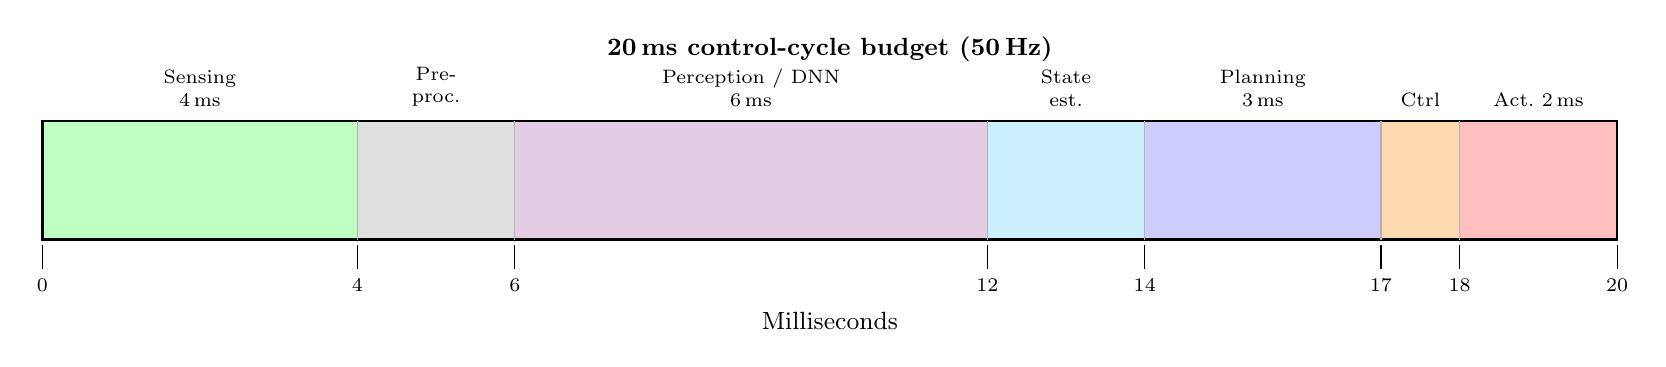
\begin{tikzpicture}[font=\scriptsize, yscale=1.5]
    \fill[green!25]  (0,0)  rectangle  (4,1);
    \fill[gray!25]   (4,0)  rectangle  (6,1);
    \fill[violet!20] (6,0)  rectangle (12,1);
    \fill[cyan!20]   (12,0) rectangle (14,1);
    \fill[blue!20]   (14,0) rectangle (17,1);
    \fill[orange!30] (17,0) rectangle (18,1);
    \fill[red!25]    (18,0) rectangle (20,1);
    \draw[thick]     (0,0)  rectangle (20,1);
    \foreach \x in {4,6,12,14,17,18}{
      \draw[gray!60, thin] (\x,0) -- (\x,1);
    }
    \node[above=2pt, align=center] at (2,1)    {Sensing\\4\,ms};
    \node[above=2pt, align=center] at (5,1)    {Pre-\\proc.};
    \node[above=2pt, align=center] at (9,1)    {Perception / DNN\\6\,ms};
    \node[above=2pt, align=center] at (13,1)   {State\\est.};
    \node[above=2pt, align=center] at (15.5,1) {Planning\\3\,ms};
    \node[above=2pt, align=center] at (17.5,1) {Ctrl};
    \node[above=2pt, align=center] at (19,1)   {Act.\ 2\,ms};
    \foreach \ms in {0,4,6,12,14,17,18,20}{
      \draw (\ms,-0.05) -- (\ms,-0.25);
      \node[below] at (\ms,-0.25) {\ms};
    }
    \node[below=12pt, font=\small] at (10,-0.25) {Milliseconds};
    \node[above=18pt, font=\small\bfseries] at (10,1)
      {20\,ms control-cycle budget (50\,Hz)};
  \end{tikzpicture}%
  }
  \caption{Visual breakdown of the 20\,ms (50\,Hz) control-cycle budget.
    Bar width is proportional to time. The \textbf{Perception/DNN} segment
    (violet) dominates; \textbf{Actuation} (red) must always be guaranteed. (Author-created figure.)}
  \label{fig:latency-bar}
\end{figure}

\subsection{Jitter, Determinism, and Priority}

Average latency hides the behavior that most often breaks controllers: variation. Jitter, cycle-to-cycle variance in completion time, matters because many control laws implicitly assume a fixed sampling period. A controller tuned for a 1\,ms loop may remain stable at 1\,ms on average and still perform poorly if the period swings between 0.8\,ms and 1.4\,ms.

Mitigating jitter is less glamorous than designing a new planner, but it is typically more decisive for safety. In practice, teams rely on priority-based scheduling, explicit CPU isolation for time-critical threads, careful memory allocation to avoid
page faults and cache thrash, and runtime choices that avoid unpredictable garbage collection on hot paths~\cite{buttazzo2011}. The challenge sharpens on heterogeneous SoCs: accelerators introduce their own scheduling queues and memory-bus contention, so variance on the GPU or NPU can propagate back into CPU-side threads unless the whole platform is treated as a coupled timing system~\cite{sze2017,casini2019}.

% ── Figure 2: hard vs soft deadlines ────────────────────────
\begin{figure}[htbp]
  \centering
  % Scale-to-fit to prevent margin overflow
  \resizebox{\linewidth}{!}{%
  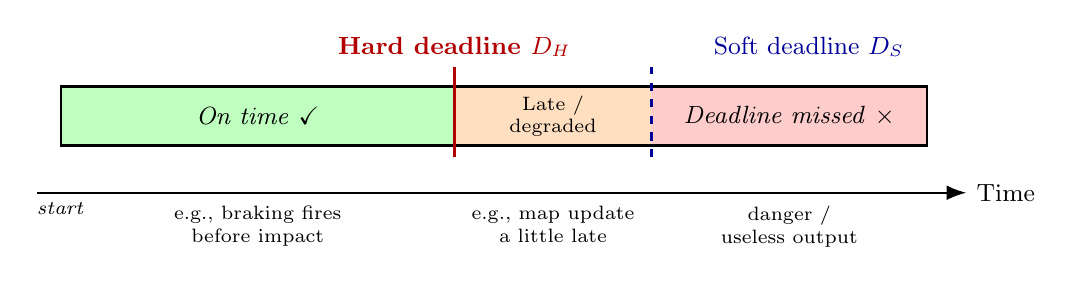
\begin{tikzpicture}[font=\small]
    \def\bh{0.75}
    \fill[green!25]  (0,0)   rectangle (5.0,\bh);
    \fill[orange!25] (5.0,0) rectangle (7.5,\bh);
    \fill[red!20]    (7.5,0) rectangle (11.0,\bh);
    \draw[thick]     (0,0)   rectangle (11.0,\bh);
    \draw[red!70!black, very thick]     (5.0,-0.15) -- (5.0,\bh+0.25);
    \draw[blue!60!black, thick, dashed] (7.5,-0.15) -- (7.5,\bh+0.25);
    \node at (2.5,  \bh/2) {\textit{On time} $\checkmark$};
    \node[font=\scriptsize, align=center] at (6.25,\bh/2) {Late /\\degraded};
    \node[align=center] at (9.25,\bh/2)  {\textit{Deadline missed} $\times$};
    \node[red!70!black, font=\small\bfseries, above] at (5.0,\bh+0.25)
      {Hard deadline $D_H$};
    \node[blue!60!black, font=\small, above] at (9.5,\bh+0.25)
      {Soft deadline $D_S$};
    \draw[-{Latex[length=2.5mm]}, thick] (-0.3,-0.6) -- (11.5,-0.6)
      node[right, font=\small] {Time};
    \node[below, font=\scriptsize] at (0,-0.6) {\textit{start}};
    \node[below, font=\scriptsize, align=center] at (2.5,-0.65)
      {e.g., braking fires\\before impact};
    \node[below, font=\scriptsize, align=center] at (6.25,-0.65)
      {e.g., map update\\a little late};
    \node[below, font=\scriptsize, align=center] at (9.25,-0.65)
      {danger /\\useless output};
  \end{tikzpicture}%
  }
  \caption{Hard vs.\ soft real-time deadlines. \textbf{Hard deadline} $D_H$
    (solid red): missing it causes unsafe outcomes. \textbf{Soft deadline}
    $D_S$ (dashed blue): late results degrade quality but remain safe.
    The red zone is always unacceptable regardless of task type. (Author-created figure.)}
  \label{fig:deadlines}
\end{figure}

\subsection{Synchronization in Multi-Sensor Fusion}

Multi-sensor fusion looks simple: ``it combines measurements to get a better estimate''. The difficulty, as teams discover in practice, is temporal. Sensors operate on separate clock domains, their acquisition pipelines have different latencies, and networked transport introduces variable delay. A fusion system that ignores these facts often produces estimates that are numerically plausible but temporally misaligned.

Three broad approaches have emerged in practice. Hardware timestamping
pushes time attribution as close to acquisition as possible. Asynchronous estimators accept out-of-sequence measurements and fuse them with explicit time models, often in Kalman-style frameworks~\cite{thrun2005}. Scheduling and observability choices can be used to prioritize sensor streams whose loss or delay would most strongly degrade safety-critical
state estimates~\cite{niu2018sensor}.

Strict sensor alignment increases sensor-to-actuator delay, whereas accepting irregular arrival reduces delay but can introduce cross-modal inconsistency. The right choice depends on what downstream controllers can tolerate and how much slack the end-to-end latency budget provides.

\begin{designbox}{Vision-centric autonomy: a case study in acceptable failure modes}
Most high-integrity robotic stacks use redundant sensing across dissimilar modalities, typically cameras, radar, and LiDAR, because heterogeneity reduces the probability that a single environmental condition disables the full perception chain. Recent surveys of autonomous-vehicle sensing emphasize that sensor selection goes beyond performance optimization: it is a design decision that shapes the
system's cost structure, operational envelope, and safety requirements~\cite{sensorlayoutreview2026,sensorsreview2026}\footnote{Reference~\cite{sensorlayoutreview2026} was in press at the time of this revision (April~2026).}.

A contrasting philosophy is to minimize the sensor suite and rely on large-scale learning to compensate for reduced geometric redundancy.  On the surface this is attractive: fewer sensors simplify calibration and integration, and the bill of materials drops.
The technical cost is subtler. With fewer independent physical cues, residual risk shifts toward the learned perception model's behavior under rare weather conditions, unusual illumination, partial occlusion, or distributional shift. Empirically, the robustness benefits of complementary modalities are visible in recent multi-modal fusion results, where camera-LiDAR-radar combinations improve generalization across conditions compared to single-modality baseline~\cite{ali2026fusion}.

For system designers, the practical takeaway is straightforward:  a vision-centric stack must compensate with stronger runtime monitoring, explicit uncertainty handling, and conservative fallback behavior, and those compensations must be justified with evidence in the safety case.
\end{designbox}

\subsection{Real-Time Machine Learning: Throughput vs.\ Worst Case}

Machine-learning models are often evaluated as if their cost is a single number: an average latency on a benchmark and an average error on a dataset. Real robots do not experience averages. They experience tails: the occasional cluttered frame, the unusual lighting condition, the burst of competing load that pushes inference from ``usually fine'' into ``occasionally late.''

This is why worst-case or tail latency matters as much as mean throughput. A model that runs in 12\,ms at the 95th percentile but stretches to 45\,ms in rare cases may be acceptable for a soft real-time perception channel and simultaneously unacceptable for any path that influences a hard real-time safety envelope. Designing for the tail becomes a distribution-shaping problem rather than a mean-shifting one.

Several families of techniques help compress the tail. Early-exit architectures can terminate computation when intermediate confidence is already sufficient. Cascades route easy inputs through lightweight classifiers and reserve heavy models for the ambiguous cases. Fixed-precision compilation and careful runtime configuration reduce numerical and memory-allocation variance, and hardware-aware scheduling disciplines such as batch size fixed to one, pre-allocation in pinned regions, reduce contention. Well-specified fallback policies matter: when a primary model misses its budget, the system must have a safe substitute that preserves the contract rather than silently violating it~\cite{sze2017,amalou2023cawet}.

% ── Figure 3: dual-path pipeline ────────────────────────────
\begin{figure}[htbp]
  \centering
  \resizebox{\linewidth}{!}{%
  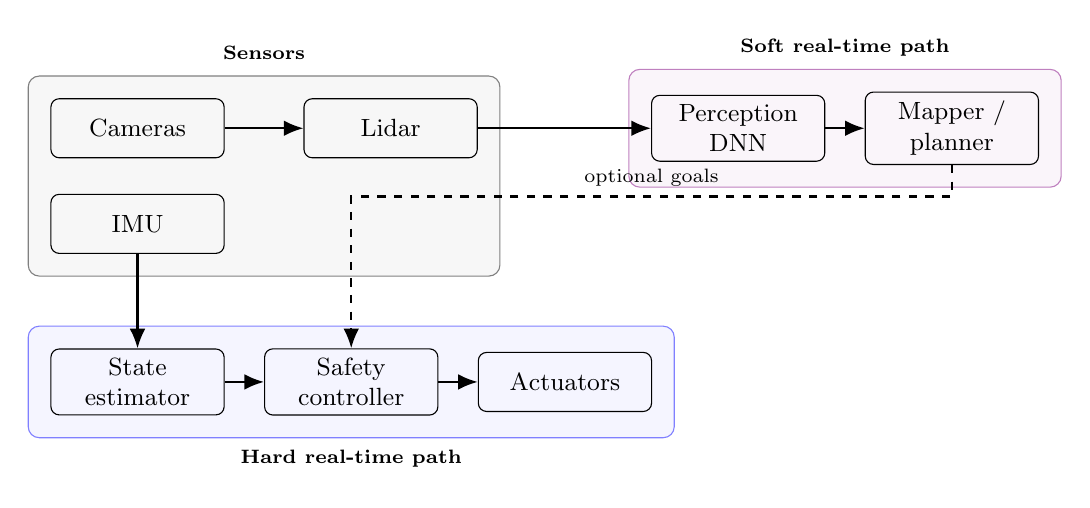
\begin{tikzpicture}[
    font=\small,
    node distance=0.45cm and 0.5cm,
    box/.style={draw, rounded corners=3pt,
                minimum width=2.2cm, minimum height=0.75cm, align=center},
    arr/.style={-{Latex[length=2.5mm,width=2mm]}, thick},
    darr/.style={-{Latex[length=2.5mm,width=2mm]}, thick, dashed}
  ]
    \node[box] (C) {Cameras};
    \node[box, below=of C] (I) {IMU};
    \node[box, right=1.0cm of C] (L) {Lidar};
    \node[box, right=2.2cm of L] (P) {Perception\\DNN};
    \node[box, right=0.5cm of P] (M) {Mapper /\\planner};
    \node[box, below=1.2cm of I] (SE) {State\\estimator};
    \node[box, right=0.5cm of SE] (SC) {Safety\\controller};
    \node[box, right=0.5cm of SC] (A) {Actuators};
    \draw[arr] (C) -- (L);
    \draw[arr] (L) -- (P);
    \draw[arr] (I) -- (SE);
    \draw[arr] (P) -- (M);
    \draw[darr] (M.south) -- ++(0,-0.4)
      -| node[near start, above, font=\scriptsize] {optional goals}
      (SC.north);
    \draw[arr] (SE) -- (SC);
    \draw[arr] (SC) -- (A);
    \begin{scope}[on background layer]
      \node[draw=black!50, rounded corners=4pt, inner sep=8pt, fill=black!3,
            fit=(C)(L)(I),
            label={[font=\scriptsize\bfseries, anchor=south]
                   north:\strut Sensors}] {};
      \node[draw=blue!50, rounded corners=4pt, inner sep=8pt, fill=blue!4,
            fit=(SE)(SC)(A),
            label={[font=\scriptsize\bfseries, anchor=north]
                   south:\strut Hard real-time path}] {};
      \node[draw=violet!50, rounded corners=4pt, inner sep=8pt, fill=violet!4,
            fit=(P)(M),
            label={[font=\scriptsize\bfseries, anchor=south]
                   north:\strut Soft real-time path}] {};
    \end{scope}
  \end{tikzpicture}}
  \caption{Dual-path architecture: a hard real-time safety loop (state estimation +
    safety controller) runs with bounded latency; perception and mapping run
    asynchronously with watchdog supervision and conservative fallbacks. (Author-created figure.)}
  \label{fig:pipeline}
\end{figure}

\subsection{Why Combining AI and Real-Time Is Structurally Difficult}
\label{subsec:ai-rt-challenge}

Real-time engineering and modern AI grew up with different success criteria. In a real-time context, the question is whether the system will meet its deadline under stress every time; in much of machine learning, the question is how the average-case error behaves on a benchmark. When these worldviews meet within a deployed robot, the mismatch manifests as a collection of ``small'' effects that interact and occasionally coalesce into a large failure.

The most obvious friction is execution-time variability. The same network can finish quickly on an easy input and stall on a cluttered one, and that variability becomes harder to bound as models become deeper and more dynamic. Worst-case inference latency for transformer-style architectures remains an open research problem, precisely because attention and memory traffic are sensitive to input structure and runtime contention~\cite{amalou2023cawet,biondi2021timepredictable}.

Less visible, but operationally important is numerical non-determinism. Parallel GPU kernels can change the order of floating-point reductions, producing outputs that are close but not identical. For perception, this is usually harmless; for safety monitors implemented as threshold tests, it can create problematic edge cases where a signal hovers around the boundary.

The harder problem is that these effects rarely occur in isolation. A perception pipeline shares caches, memory bandwidth, and sometimes even power and thermal headroom with control and communication threads. Under load, contention-driven jitter can propagate into the very layer that must stay deterministic, unless cores, memory, and execution budgets are deliberately partitioned.

Learned components are also difficult to justify to external assurance processes. When a controller is specified as code plus a proof obligation, failures can be traced to violated assumptions. When behavior is embodied in weights, the same diagnostic story is harder to tell, yet regulators increasingly expect such structured explanations~\cite{brunke2022,seshia2022}.

\subsection{Worked Example: Temporal Layers in an Autonomous Vehicle}
\label{subsec:av-example}

Timescale separation is how a well-engineered autonomous vehicle handles these tensions. At the lowest layer, running at 1\,000\,Hz with microsecond deadlines, brake and steering controllers read wheel-speed sensors and adjust hydraulic pressure; these loops are implemented on dedicated real-time hardware and intentionally isolated from the software stacks above them. At 100\,Hz, a sensor fusion layer integrates camera frames, LiDAR, radar, and GPS into a unified world picture with hard real-time guarantees on its own output latency. At 10\,Hz, a prediction and motion planning layer evaluates candidate paths given the world state from fusion; planning uses predictive models with a longer compute budget because the output is consumed asynchronously by the control layer. At roughly 1\,Hz, a behavioral planner makes slower maneuver and route decisions. Asynchronously in the background, a cloud connection downloads updated map tiles and improved model weights.

The structural key is that no layer waits for the layer above it. If the behavioral planner consumes an extra 500\,ms, the motor controllers and sensor fusion layer continue operating correctly because they hold the most recent valid goal and execute against it. This non-blocking, timescale-separated hierarchy is the canonical pattern for real-time intelligence in mobile autonomous systems, and its integrity depends on lower layers having fallback behaviors that remain safe in the absence of fresher higher-level guidance.
% =============================================================================
\section{Scalable Architecture for Robotics}
\label{sec:scale}

Robotic scalability spans at least four independent dimensions: compute capacity per robot, communication bandwidth and latency within and across robots, organizational modularity that allows teams to evolve subsystems independently, and verification coverage that does not collapse as system complexity grows. A design that works well for a single robot in a controlled lab tends to fail in at least five observable ways as deployment scope expands, each requiring deliberate architectural decisions rather than incremental performance tuning.

\subsection{Five Dimensions of Growth}

Robotic systems ``scale'' along more than one axis, and the axes interact. A design change that appears harmless in a single-robot prototype can become the dominant bottleneck once the same code is replicated across a fleet.

One axis is \emph{sensor complexity}.  Moving from a single camera to a multi-modal suite, cameras, inertial sensors, and ranging, increase not only bandwidth but also synchronization work and fusion latency. A second axis is \emph{task complexity}. Point-to-point navigation assumes relatively stable environments, whereas operation in human spaces forces planners to account for uncertainty, congestion, and social constraints, all of which increase the state space and replanning frequency.

A third axis is \emph{fleet scale}.  Coordination overhead grows nonlinearly because communication, shared-map consistency, and contention for shared infrastructure such as SLAM services or dispatch servers, introduce tail-latency effects that do not appear in small-team tests. The remaining two axes are tied to learning. First, \emph{computational demand} has risen with modern perception models, making the robot's thermal and power envelope a real-time consideration. Second, \emph{geographic scope} introduces wide-area links and intermittent connectivity, which means the architecture must degrade gracefully. Local safety loops must remain deterministic even when global services are slow or unreachable.

\subsection{Layered and Hierarchical Control}

A common architectural answer to the ``fast versus smart'' tension is to separate functions by timescale. Hierarchical control isolates the reactive safety layer, the part that must respond within milliseconds and can be analyzed as hard real-time, from deliberative layers that optimize over seconds or minutes and can therefore tolerate longer compute budgets~\cite{brooks1986}.

Brooks's subsumption architecture offered an early, influential expression of this principle. Modern stacks look different in detail, but they preserve the same invariant: overload or failure in a higher layer must not be able to stall, starve, or otherwise compromise the guarantees of the lowest safety-critical layer. When that invariant is violated, architectural complexity turns directly into timing risk.

% ── Figure 4: three-layer hierarchy ─────────────────────────
\begin{figure}[htbp]
  \centering
  \resizebox{\linewidth}{!}{%
  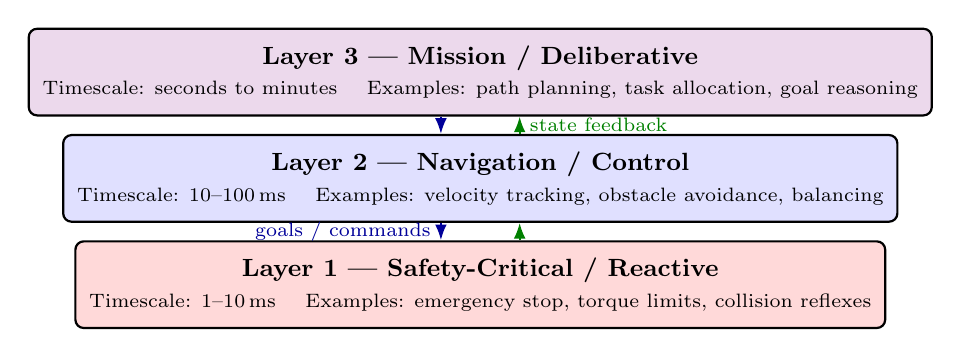
\begin{tikzpicture}[font=\small]
    \def\lw{10.0cm}
    \def\lh{1.10cm}
    \node[draw, thick, fill=violet!15, minimum width=\lw, minimum height=\lh,
          rounded corners=3pt, align=center, inner sep=5pt]
      (L3) at (0, 2.70) {
        \textbf{Layer 3 --- Mission / Deliberative}\\
        {\scriptsize Timescale: seconds to minutes \quad
         Examples: path planning, task allocation, goal reasoning}};
    \node[draw, thick, fill=blue!12, minimum width=\lw, minimum height=\lh,
          rounded corners=3pt, align=center, inner sep=5pt]
      (L2) at (0, 1.35) {
        \textbf{Layer 2 --- Navigation / Control}\\
        {\scriptsize Timescale: 10--100\,ms \quad
         Examples: velocity tracking, obstacle avoidance, balancing}};
    \node[draw, thick, fill=red!15, minimum width=\lw, minimum height=\lh,
          rounded corners=3pt, align=center, inner sep=5pt]
      (L1) at (0, 0) {
        \textbf{Layer 1 --- Safety-Critical / Reactive}\\
        {\scriptsize Timescale: 1--10\,ms \quad
         Examples: emergency stop, torque limits, collision reflexes}};
    \draw[-{Latex[length=2mm]}, thick, blue!60!black]
      ([xshift=-0.5cm] L3.south) -- ([xshift=-0.5cm] L2.north);
    \draw[-{Latex[length=2mm]}, thick, blue!60!black]
      ([xshift=-0.5cm] L2.south) -- ([xshift=-0.5cm] L1.north)
      node[midway, left, font=\scriptsize] {goals / commands};
    \draw[-{Latex[length=2mm]}, thick, dashed, green!50!black]
      ([xshift=0.5cm] L1.north) -- ([xshift=0.5cm] L2.south);
    \draw[-{Latex[length=2mm]}, thick, dashed, green!50!black]
      ([xshift=0.5cm] L2.north) -- ([xshift=0.5cm] L3.south)
      node[midway, right, font=\scriptsize] {state feedback};
  \end{tikzpicture}}
  \caption{Three-layer hierarchical control architecture. Layer~1 (red) provides hard
    real-time guarantees: it responds within 1--10\,ms regardless of the higher layers.
    Goals flow \emph{downward} (solid); state feedback flows \emph{upward} (dashed).
    If a higher layer crashes, lower layers continue to guarantee basic safety. (Author-created figure.)}
  \label{fig:layers}
\end{figure}

\subsection{Middleware, QoS, and Discovery}

Middleware is where architectural intent meets transport reality. Publish-subscribe abstractions only become useful when the runtime provides concrete controls over reliability, buffering, and delivery semantics. ROS~2 exposes these controls through DDS QoS policies tuned to robotic timing and reliability requirements~\cite{maruyama2016,kronauer2021}.

In this context, ``more reliable'' is not always ``better.'' A high-rate camera stream often benefits from best-effort delivery with volatile durability: dropping an occasional frame is typically preferable to back-pressure that inflates latency. Command and safety channels invert that trade-off. If a velocity command is lost, the robot can enter an indeterminate state, so reliable delivery and
careful queue sizing become part of the safety argument. Table~\ref{tab:qos} collects representative combinations that recur in deployed systems.

\begin{table}[htbp]
  \centering
  \caption{Common ROS~2 QoS policy combinations and recommended use cases.}
  \label{tab:qos}
  \rowcolors{2}{tablealt}{white}
  \renewcommand{\arraystretch}{1.15}
  \begin{tabular}{@{}L{0.26\linewidth}L{0.13\linewidth}L{0.17\linewidth}L{0.33\linewidth}@{}}
    \toprule
    \rowcolor{tablehead}
    \textcolor{white}{\textbf{Channel type}} &
    \textcolor{white}{\textbf{Reliability}} &
    \textcolor{white}{\textbf{Durability}} &
    \textcolor{white}{\textbf{Typical use case}} \\
    \midrule
    Sensor stream (camera, lidar) & Best-effort & Volatile &
      High-rate data; Occasional dropped frame is acceptable \\
    Velocity / command & Reliable & Volatile &
      Must not lose messages; delivery order matters \\
    Parameters / config & Reliable & Transient-local &
      Late-joining nodes receive the last stored value \\
    Diagnostics / health & Best-effort & Volatile &
      Lightweight; occasional loss acceptable \\
    Map / occupancy grid & Reliable & Transient-local &
      Large payload; new subscribers need the current map \\
    \bottomrule
  \end{tabular}
  \renewcommand{\arraystretch}{1}
\end{table}

\subsection{Horizontal Scaling: Multi-Robot and Swarms}

Fleet coordination reveals scaling limits quickly. Once the number of robots grows, a single planner is asked to do two incompatible jobs: maintain global situational awareness and respond within tight latency bounds. At that point, centralization turns into both a bottleneck and a single point of failure.

Partially distributed approaches give up some global optimality at the expense of throughput and robustness. Market-based allocation, distributed MPC, and consensus protocols represent different points in that trade space~\cite{gerkey2004}. In
warehouse-style settings, auction mechanisms are attractive because their per-task computation can scale well and because they gracefully degrade as robots join, leave, or fail.

Coordination is not ``just an algorithm'' layer: it is an architectural choice that shapes tail latency under load. Table~\ref{tab:coord} summarizes these paradigms with an explicit focus on those trade-offs.

\begin{table}[htbp]
  \centering
  \caption{Comparison of coordination paradigms (qualitative).}
  \label{tab:coord}
  \rowcolors{2}{tablealt}{white}
  \renewcommand{\arraystretch}{1.15}
  \begin{tabular}{@{}L{0.24\linewidth}L{0.32\linewidth}L{0.30\linewidth}@{}}
    \toprule
    \rowcolor{tablehead}
    \textcolor{white}{\textbf{Paradigm}} &
    \textcolor{white}{\textbf{Strengths}} &
    \textcolor{white}{\textbf{Risks / costs}} \\
    \midrule
    Centralized planner   & Global optimality (small teams) & Single point of failure \\
    Hierarchical          & Clear command structure & Interface rigidity \\
    Distributed consensus & Robustness; no central brain & Slower convergence \\
    Learning-based        & Handles messy environments & Data hunger; hard to verify \\
    \bottomrule
  \end{tabular}
  \renewcommand{\arraystretch}{1}
\end{table}

\subsection{Vertical Scaling: From Embedded to Cloud}

Vertical scaling concerns what the robot can do with the compute and power it carries. For many platforms, perception is the limiting workload: models must deliver adequate accuracy while staying inside tight thermal and battery envelopes. As transformer-based architectures have increased computational demand, the gap between cloud-scale training hardware and edge deployment hardware has widened, and performance now depends on co-design choices such as quantization, structured sparsity, and operator fusion~\cite{sze2017}.

Heterogeneous SoCs address this by combining CPUs, GPUs, and neural accelerators into a single package. Used well, an accelerator can provide lower variance than general-purpose GPU execution because it reduces contention and constrains the runtime behavior more tightly. Used poorly, it simply adds another queue and another point of contention.

Table~\ref{tab:edgecloud} summarizes the practical trade-offs when these design choices
are pushed across the edge--fog--cloud tiers.

\begin{table}[htbp]
  \centering
  \caption{Edge--cloud deployment trade-offs.}
  \label{tab:edgecloud}
  \rowcolors{2}{tablealt}{white}
  \renewcommand{\arraystretch}{1.15}
  \begin{tabular}{@{}L{0.18\linewidth}L{0.19\linewidth}L{0.23\linewidth}L{0.25\linewidth}@{}}
    \toprule
    \rowcolor{tablehead}
    \textcolor{white}{\textbf{Dimension}} &
    \textcolor{white}{\textbf{On-robot}} &
    \textcolor{white}{\textbf{Fog / on-prem}} &
    \textcolor{white}{\textbf{Cloud}} \\
    \midrule
    Typical latency     & $<5$\,ms           & 5--50\,ms          & 50--500\,ms \\
    Compute power       & Low -- medium      & Medium -- high     & Very high \\
    Connectivity needed & None               & Local network      & Internet \\
    Best suited for     & Safety reactions   & Fleet coordination & Model training \\
    Main risk           & Limited RAM/GPU    & LAN outage         & High delay \\
    \bottomrule
  \end{tabular}
  \renewcommand{\arraystretch}{1}
\end{table}

\subsection{Temporal Intelligence Contract (TIC)}
\label{sec:tic}

Existing approaches to system contracts in distributed software, service level agreements, interface description languages, and component-based design notations, handle functional correctness and availability well but leave timing, uncertainty, and safety-specific degradation behaviors unaddressed. This work introduces the \textbf{Temporal Intelligence Contract (TIC)}, a reference-specification that goes beyond static documentation to one that can be audited and automatically monitored at runtime. 

A TIC is a machine-readable contract that holds each component to five obligations. The \textbf{latency envelope} specifies best-case, typical, and worst-case completion times on the actual deployment hardware, measured under realistic concurrent load, not under ideally isolated conditions. The \textbf{uncertainty envelope} defines calibration requirements and the maximum distributional drift the system will tolerate before downstream safety logic stops trusting the component's predictions. The \textbf{safety fallback policy} prescribes degraded-mode and emergency-stop behaviors triggered when other clauses are violated, captured as a formal state machine that operates without human intervention. The \textbf{observability payload} defines the traces, timing counters, and health probes the component must emit continuously for contract verification during operation. The \textbf{scalability clause} caps fan-out, topic publication rates, and admission-control behaviors under load, preventing a misbehaving component from propagating back-pressure through the system.

Unlike a static requirement specification, TIC treats its obligations as \emph{operational claims} that must remain true at runtime. That orientation changes how teams build systems. Instead of treating timing and safety as properties established once during integration testing, TIC assumes conditions will drift, through thermal throttling, network contention, sensor degradation, and workload changes, and requires the system to detect drift early enough to stay safe.

Consider a warehouse AMR whose local perception module publishes obstacle detections at 30\,Hz. A classical interface description would specify message fields and perhaps an update rate. A TIC also binds the module to (i) a worst-case end-to-end detection latency on the target SoC, (ii) an uncertainty calibration requirement, such as confidence scores remaining calibrated under the site's lighting conditions, and (iii) a specific degraded behavior when those claims stop being true, such as reducing speed, widening stop distances, or entering a supervised mode. The fallback is not informal ``operator will handle it'' assumption; it is part of the machine-executable contract. A complete structured schema and
{JSON} schema for {TIC} clause instantiation is beyond the scope of this paper; the clause structure in Table~\ref{tab:tic} defines the required fields and types sufficient for conforming implementation.

Runtime monitoring also changes failure analysis. When an incident occurs, TIC-style telemetry provides a structured record of whether deadlines were being approached, whether uncertainty was drifting, and whether back-pressure was building in the communication graph. This gives the missing connective tissue between learning-system behavior and the evidence that a safety case demands.

The violation penalty term \(P_v\) is defined as the ratio
of contract-violation events to total monitored cycles:
\(P_v = N_{\text{violations}} / N_{\text{cycles}}\);
for the example in Table~6, \(P_v = 3/60 = 0.05\).

The RTI-Score provides a deployment-readiness metric that aggregates compliance across clauses:
\[
  \mathrm{RTI\text{-}Score}
  = w_1 S_t + w_2 S_q + w_3 S_s + w_4 S_o - w_5 P_v
\]

The linear aggregation form is proposed as a design pattern; the weights $w_1$--$w_5$ are not universal constants and must be calibrated for each deployment through system-level hazard analysis (FMEA or HAZOP), consistent with the applicable safety standard (ISO 26262, IEC 61508, or ISO 10218).

\vspace{4pt}
\noindent\fbox{\parbox{0.98\linewidth}{\footnotesize\textbf{NOTE:} The weights $w_1\!=\!0.15$, $w_2\!=\!0.15$, $w_3\!=\!0.35$, $w_4\!=\!0.10$, $w_5\!=\!0.25$ used below are solely to demonstrate arithmetic; they carry no engineering authority. For any deployment, weights \emph{must} be derived through system-level hazard analysis (FMEA or HAZOP) against the applicable safety standard (ISO 26262, IEC 61508, or ISO 10218). Using illustrative weights in a production system without this analysis constitutes an unsafe practice.}}
\vspace{4pt}

The term values in Table~\ref{tab:rti_example} are illustrative and do not derive from physical deployment; they demonstrate the scoring mechanics only.

\begin{table}[htbp]
  \centering
  \caption{Worked example of RTI-Score computation for an AMR perception module over a 60-cycle monitoring window. Values are illustrative; they demonstrate the scoring mechanics and are not derived from physical deployment.}
  \label{tab:rti_example}
  \rowcolors{2}{tablealt}{white}
  \renewcommand{\arraystretch}{1.15}
  \begin{tabular}{@{}L{0.22\linewidth}C{0.12\linewidth}L{0.55\linewidth}@{}}
    \toprule
    \rowcolor{tablehead}
    \textcolor{white}{\textbf{Term}} &
    \textcolor{white}{\textbf{Value}} &
    \textcolor{white}{\textbf{Rationale}} \\
    \midrule
    $S_t$ (timing compliance)      & 0.92 & 92\% of deadlines met in window \\
    $S_q$ (task quality)           & 0.87 & Detection F1\,=\,0.87 on deployment distribution \\
    $S_s$ (safety compliance)      & 1.00 & No safety-fallback triggers in window \\
    $S_o$ (observability)          & 0.78 & 22\% of expected telemetry traces missing \\
    $P_v$ (violation penalty)      & 0.05 & 3 minor contract violations in window \\
    \bottomrule
  \end{tabular}
  \renewcommand{\arraystretch}{1}
  \vspace{2pt}
  \caption*{\footnotesize With $w_1\!=\!0.15$, $w_2\!=\!0.15$, $w_3\!=\!0.35$,
    $w_4\!=\!0.10$, $w_5\!=\!0.25$: RTI-Score $= 0.138 + 0.131 + 0.350 +
    0.078 - 0.013 = 0.684$.}
\end{table}

\FloatBarrier

Weights $w_i$ are application-specific and must be determined
during system-level hazard analysis, such as FMEA or HAZOP,
consistent with safety standards such as ISO~26262,
IEC~61508, or ISO~10218; $w_3$ and $w_5$ typically carry the highest values
because safety compliance and violation penalties take priority
over throughput. A module whose RTI-Score drops below a
deployment-specified threshold can be quarantined for
investigation without bringing down the wider system.

\subsubsection{Worked FMEA grounding for RTI-Score weights (illustrative)}
\label{subsec:fmea_weights}
To reduce ``numerology'' risk in weight selection, a minimal Failure Modes and Effects
Analysis (FMEA) can be used to map dominant hazards to TIC clauses and to derive weight
priors. Table~\ref{tab:fmea} illustrates this for a warehouse AMR perception pipeline.
Each failure mode is scored by Severity (S), Occurrence (O), and Detectability (D) on a
1--10 scale, producing a Risk Priority Number (RPN \(=S\times O\times D\)). RPN mass is
then allocated to TIC clause families; weights \(w_i\) are set proportional to those
allocations (and must be reviewed by the responsible safety process owner).

\begin{table}[htbp]
  \centering
  \caption{Illustrative FMEA for a warehouse AMR perception path and mapping to TIC clauses (example only; replace with deployment-specific scoring).}
  \label{tab:fmea}
  \rowcolors{2}{tablealt}{white}
  \renewcommand{\arraystretch}{1.15}
  \setlength{\tabcolsep}{3pt}
  \begin{tabular}{@{}L{0.26\linewidth}L{0.26\linewidth}C{0.06\linewidth}C{0.06\linewidth}C{0.06\linewidth}C{0.08\linewidth}L{0.16\linewidth}@{}}
    \toprule
    \rowcolor{tablehead}
    \textcolor{white}{\textbf{Failure mode}} &
    \textcolor{white}{\textbf{Effect}} &
    \textcolor{white}{\textbf{S}} &
    \textcolor{white}{\textbf{O}} &
    \textcolor{white}{\textbf{D}} &
    \textcolor{white}{\textbf{RPN}} &
    \textcolor{white}{\textbf{Primary TIC clause}} \\
    \midrule
    Perception deadline misses under load & Late obstacle updates; unsafe braking margin & 9 & 4 & 4 & 144 & Latency envelope / penalty \\
    Confidence miscalibration & False safe states; unsafe speed selection & 9 & 3 & 6 & 162 & Uncertainty envelope \\
    Distributional drift (lighting/reflective floors) & Degraded detection quality; near-miss risk & 8 & 4 & 5 & 160 & Drift envelope / fallback \\
    Fallback not triggered when needed & Unsafe continuation in violated state & 10 & 2 & 6 & 120 & Safety fallback \\
    Missing telemetry/trace gaps & Inability to audit and diagnose violations & 6 & 4 & 7 & 168 & Observability payload \\
    Queue growth/back-pressure cascade & Latency amplification across graph & 7 & 3 & 5 & 105 & Scalability clause \\
    \bottomrule
  \end{tabular}
  \renewcommand{\arraystretch}{1}
\end{table}

\noindent\textbf{Weight derivation (example).} Aggregating RPN by clause family yields a
prioritization in which safety/fallback and violation penalty are dominant, followed by
timing and observability, with task-quality weighted lower unless the mission is
efficiency-critical. In practice, teams can normalize clause-RPN totals to define initial
\(w_i\) values, then calibrate against field evidence and safety targets.

\FloatBarrier

\begin{table}[htbp]
  \centering
  \caption{TIC clauses for multi-tier robotic systems.}
  \label{tab:tic}
  \rowcolors{2}{tablealt}{white}
  \renewcommand{\arraystretch}{1.15}
  \begin{tabular}{@{}L{0.19\linewidth}L{0.25\linewidth}L{0.22\linewidth}L{0.22\linewidth}@{}}
    \arrayrulecolor{black}\toprule
    \rowcolor{tablehead}
    \textcolor{white}{\textbf{TIC clause}} &
    \textcolor{white}{\textbf{Required artifact}} &
    \textcolor{white}{\textbf{Runtime check}} &
    \textcolor{white}{\textbf{Typical owner}} \\
    \midrule
    Latency envelope     & Deadline profile per path        & Deadline miss ratio & RT engineer \\
    Uncertainty envelope & Calibration report, OOD threshold & Confidence drift    & ML engineer \\
    Safety fallback      & State machine for degrade/stop    & Trigger rate        & Safety engineer \\
    Observability payload& Trace schema, metrics contract    & Missing telemetry   & DevOps / SRE \\
    Scalability clause   & Rate limits, backpressure policy  & Queue depth         & Platform architect \\
    \bottomrule
  \end{tabular}
  \renewcommand{\arraystretch}{1}
\end{table}

\FloatBarrier

\subsubsection{Reference TIC schema and monitoring semantics}
\label{sec:tic_schema}

To make TIC implementable and auditable, a conforming component SHOULD publish a
versioned contract document (e.g., JSON) and a runtime ``contract status'' stream.
The document defines static intent (thresholds, deadlines, ownership); the status
stream provides the time-indexed evidence used for compliance.

\begin{table}[htbp]
  \centering
  \small
  \caption{Compact TIC contract schema excerpt (illustrative).}
  \label{tab:tic_schema_excerpt}
  \rowcolors{2}{tablealt}{white}
  \renewcommand{\arraystretch}{1.15}
  \begin{tabular}{@{}L{0.30\linewidth}L{0.18\linewidth}L{0.42\linewidth}@{}}
    \toprule
    \rowcolor{tablehead}
    \textcolor{white}{\textbf{Field}} &
    \textcolor{white}{\textbf{Type}} &
    \textcolor{white}{\textbf{Meaning}} \\
    \midrule
    tic\_version & string & Contract schema version (semver). \\
    component.name & string & Component identifier (node/service). \\
    component.build & string & Immutable build provenance (git hash/image tag). \\
    time\_base & string & Clock source for timestamps (e.g., monotonic). \\
    paths[*].deadline\_ms & number & Deadline per monitored end-to-end path. \\
    paths[*].latency\_env\_ms & object & p50/p95/p99/max under declared conditions. \\
    uncertainty.cal\_metric & string & Calibration metric name (e.g., ECE). \\
    uncertainty.drift\_metric & string & Drift metric name (e.g., PSI, MMD). \\
    fallback.state\_machine & string & Named fallback policy/state machine. \\
    observability.metrics & array & Metrics/traces the component must emit. \\
    scalability.publish\_rate\_max & number & Declared rate ceiling to prevent back-pressure. \\
    \bottomrule
  \end{tabular}
  \renewcommand{\arraystretch}{1}
\end{table}

\begin{designbox}{Minimal TIC contract example (illustrative JSON)}
\begin{verbatim}
{
  "tic_version": "1.0",
  "component": {
    "name": "perception_node",
    "build": "git:abc123"
  },
  "critical_paths": [
    {
      "path_id": "camera->detections",
      "deadline_ms": 25.0,
      "latency_envelope_ms": {
        "p50": 8.0,
        "p95": 14.0,
        "p99": 20.0,
        "max": 25.0
      }
    }
  ],
  "uncertainty": {
    "calibration_metric": "ECE",
    "ece_max": 0.05,
    "drift_metric": "PSI",
    "drift_warn": 0.20,
    "drift_violate": 0.35
  },
  "fallback": {
    "state_machine": "TIER_DOWN_OR_STOP",
    "max_consecutive_deadline_misses": 2
  },
  "observability": {
    "required_metrics": ["latency_hist", "deadline_miss", "queue_depth"],
    "min_emit_hz": 1.0
  },
  "scalability": {
    "publish_rate_hz_max": 30,
    "queue_depth_max": 10,
    "backpressure_policy": "drop_oldest"
  }
}
\end{verbatim}
\end{designbox}

\noindent\textbf{Monitoring semantics (required).} A TIC monitor MUST specify: (i)
window definition (e.g., last $N$ cycles or $T$ seconds), (ii) the exact test for
``deadline miss'' (e.g., end-to-end timestamping boundaries), (iii) how uncertainty
and drift metrics are computed and rate-limited, and (iv) how violations are
aggregated into triggers for the fallback state machine. For example, Expected
Calibration Error (ECE) is a standard calibration summary metric~\cite{guo2017calibration}.
Population Stability Index (PSI), commonly used in credit risk monitoring, is one
simple drift indicator~\cite{siddiqi2005scorecards}; alternatives include kernel MMD~\cite{gretton2012kernel}
and streaming change detectors such as ADWIN~\cite{bifet2007adwin}.

\noindent\textbf{Conformance checklist (minimum).} A TIC-conforming component MUST:
(1) expose deadlines/paths with units; (2) emit per-window miss statistics; (3)
emit the uncertainty/drift signals named in the contract; (4) expose the current
fallback state; and (5) enforce the declared scalability limits (rate/queue/fan-out)
locally, not as a best-effort operator procedure.

% ── Figure 5: edge-cloud split ───────────────────────────────
\begin{figure}[htbp]
  \centering
  \resizebox{0.96\linewidth}{!}{%
  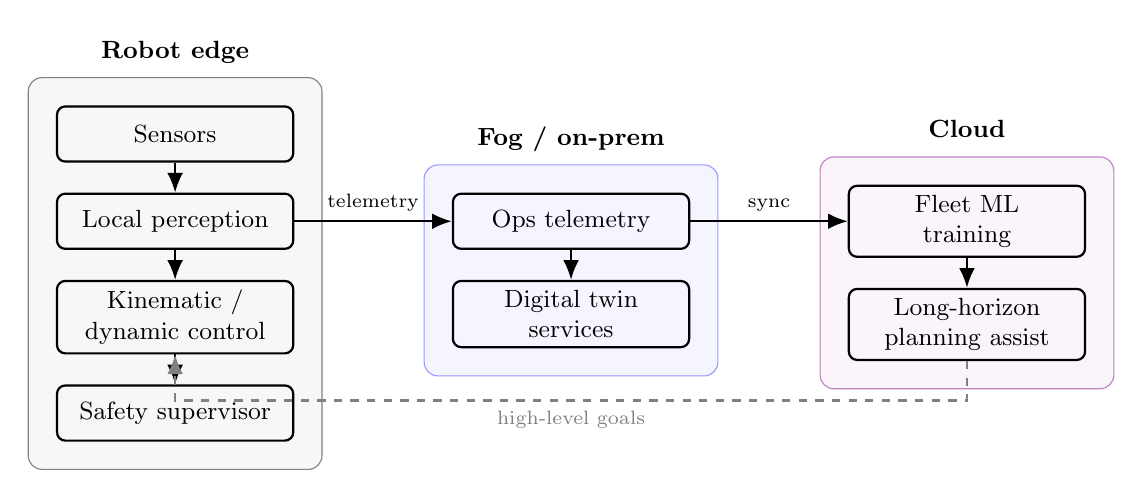
\begin{tikzpicture}[
    font=\small,
    node distance=0.38cm and 2.0cm,
    box/.style={draw, thick, rounded corners=3pt,
                minimum width=3.0cm, minimum height=0.7cm, align=center},
    arr/.style={-{Latex[length=2.5mm,width=2mm]}, thick},
    darr/.style={-{Latex[length=2.5mm,width=2mm]}, thick, dashed, gray}
  ]
    \node[box] (S)  {Sensors};
    \node[box, below=of S]  (LP) {Local perception};
    \node[box, below=of LP] (K)  {Kinematic /\\dynamic control};
    \node[box, below=of K]  (SF) {Safety supervisor};
    \node[box, right=of LP] (OT) {Ops telemetry};
    \node[box, below=of OT] (DT) {Digital twin\\services};
    \node[box, right=of OT] (FM)  {Fleet ML\\training};
    \node[box, below=of FM] (MAP) {Long-horizon\\planning assist};
    \begin{scope}[on background layer]
      \node[draw=black!50, rounded corners=5pt, inner sep=10pt, fill=black!3,
            fit=(S)(LP)(K)(SF),
            label={[font=\small\bfseries, anchor=south]
                   north:\strut Robot edge}] (R) {};
      \node[draw=blue!40, rounded corners=5pt, inner sep=10pt, fill=blue!4,
            fit=(OT)(DT),
            label={[font=\small\bfseries, anchor=south]
                   north:\strut Fog / on-prem}] (F) {};
      \node[draw=violet!50, rounded corners=5pt, inner sep=10pt, fill=violet!4,
            fit=(FM)(MAP),
            label={[font=\small\bfseries, anchor=south]
                   north:\strut Cloud}] (CL) {};
    \end{scope}
    \draw[arr] (S)  -- (LP);
    \draw[arr] (LP) -- (K);
    \draw[arr] (K)  -- (SF);
    \draw[arr] (OT) -- (DT);
    \draw[arr] (FM) -- (MAP);
    \draw[arr] (LP) -- node[above, font=\scriptsize] {telemetry} (OT);
    \draw[arr] (OT) -- node[above, font=\scriptsize] {sync} (FM);
    \draw[darr]
      (MAP.south) -- ++(0,-0.5)
      -| node[near start, below, font=\scriptsize] {high-level goals}
      (K.south);
  \end{tikzpicture}}
  \caption{Typical edge-cloud split: closed-loop safety and actuation remain on-robot; fleet analytics and training reside off-robot with asynchronous interaction. Solid arrows: real-time data flow. Dashed arrow: asynchronous goal delivery from cloud planner to on-robot kinematic controller.}
  \label{fig:edgecloud}
\end{figure}

\subsection{Worked Example: Scaling a Warehouse Robot Fleet}

A warehouse fleet provides a revealing stress test because scaling tends to happen in clear inflection points. Imagine a team that starts with five robots and grows to two hundred over a few years. Early on, a flat task-assignment module may appear
sufficient because the system rarely experiences contention. As the fleet approaches a few dozen units, however, that same module becomes a latency bottleneck; replacing it with an auction-style allocator restores assignment responsiveness without forcing
changes elsewhere, provided the interface boundaries were designed well~\cite{wurman2008}.

Shared perception infrastructure typically becomes the next constraint. When each robot streams sensor data to a central SLAM service, the service can saturate before any individual robot appears overloaded. Splitting SLAM into per-zone edge instances and synchronizing map segments asynchronously reduces tail latency and prevents congestion in one zone from propagating across the fleet.

Outages then test whether the system is resilient or merely fast. When a network partition isolates a warehouse zone, robots must fall back to local navigation with conservative obstacle avoidance. Across all of these transitions, the core discipline is separation of concerns: the 1\,000\,Hz motor controller and safety interlocks remain stable regardless of what happens in task allocation and fleet coordination above them.

% =============================================================================
\section{Integrating Learning Without Breaking Time}
\label{sec:learn}

\subsection{Model Lifecycle and Real-Time Inference}

A production learning pipeline for robotics extends well beyond training. It includes how data is collected and governed, how models are validated against representative operational conditions, how releases are staged, and how rollbacks are executed when field performance drifts.

What makes robotics distinct is that learning runs in a closed loop. Predictions change actions; actions change what the robot sees next; and the logged data that feeds the next training cycle is therefore shaped by the current model's biases~\cite{ross2011}.
A navigation policy that is slightly over-confident in one corner case can steer the robot into trajectories that over-represent that corner case, slowly shifting the training distribution away from the scenarios that the system must handle safely.

For that reason, monitoring is not a ``nice-to-have'' add-on. Detecting distributional shift early, before it accumulates into a safety-relevant degradation, requires instrumentation that is designed in and maintained over time. This is exactly the motivation behind the TIC uncertainty-envelope and observability clauses: they turn monitoring expectations into explicit obligations rather than best-effort practice.

\subsection{Fleet-Scale Learning}

Fleet-scale deployment turns learning into an operational systems problem. Once a
robotic product runs as a fleet, it starts to encounter the long tail of rare
conditions at a pace that no lab campaign can match. The implication is that model
improvement depends as much on the data and evaluation pipeline as on the model class
itself. Recent work on shared fleet learning emphasizes both the
benefits of aggregated experience and the constraints it
introduces, including privacy, annotation cost, governance,
and validation burden~\cite{retory2021federated}.
Large-scale autonomous driving datasets further demonstrate
the value of aggregated experience for learning-based
perception in complex environments~\cite{sun2020waymo}.

Fleet learning must be designed as part of the real-time system. Logging budgets, data transport, and release mechanisms are not free; they compete with on-device compute, storage, and bandwidth. TIC-style clauses provide a practical way to make those costs explicit: observability and scalability requirements can be stated, monitored, and enforced rather than assumed.

Fleet learning also introduces verification asymmetry. A modular pipeline can often be tested component-by-component with interpretable intermediate signals. End-to-end learning reduces hand-built interfaces, but it can also reduce debuggability when a
failure occurs because the system offers fewer ``hooks'' for diagnosis. It pushes more of the assurance burden onto monitoring, regression test design, and evidence collection, and it makes safety case construction more demanding when the certified unit is an opaque network rather than a specified control law~\cite{seshia2022,brunke2022}. In that sense, the modular and end-to-end approaches are not a simple quality ladder;
they are different engineering bets with different evidence requirements and different failure modes.

\subsection{Simulation and Digital Twins}

Simulation has shifted from convenience to a necessity in modern robotics. When collecting real-world data is expensive, slow, or dangerous, a high-fidelity simulator can generate repeatable conditions for debugging and for stress-testing policies
against rare scenarios that would be irresponsible to stage physically~\cite{shah2018airsim}.

The value of simulation, however, is bounded by the sim-to-real gap. Rendering and physics engines cannot perfectly reproduce sensor noise, contact dynamics, or the long-tail interactions that occur in deployed environments. Domain randomization and
adaptation reduce this gap, but they do not eliminate it; the practical response is to treat simulation results as evidence that must be calibrated against field behavior using explicit validation protocols~\cite{tobin2017domain,zhao2020sim2real}.

Digital twins extend the idea beyond pre-deployment testing. Instead of being a standalone scenario generator, a twin becomes a continuously updated operational model used for monitoring, anomaly detection, and predictive maintenance at scale.

\subsection{Contract-Aware Adaptive Inference (CAAI)}
\label{sec:caai}

The TIC framework defines the obligations; CAAI is a concrete way to satisfy them in a perception stack that must run under changing conditions. The motivating observation is simple but easy to ignore during development: no single model choice maximizes accuracy, minimizes worst-case latency, and minimizes compute cost at the same time. On finite hardware, those objectives conflict, and the conflict is sharpest exactly
when the robot is stressed, in crowded scenes, degraded sensing, network load, thermal throttling, or other competing activity.
CAAI treats perception quality as a \emph{managed resource}. Rather than locking in a single operating point, it runs a small family of models: a full-resolution model that provides the best quality when budget allows, a compressed model that reduces compute and variance, and an emergency tier whose outputs are minimal but whose completion time is compatible with the safety-critical budget. Conceptually this is aligned with anytime algorithms and imprecise computation models, where result quality is traded against time/compute under explicit control~\cite{deanboddy1988,zilberstein1996anytime,shihliu1995}.

The key engineering choice is that switching in CAAI is predictable by design, rather than opportunistic. A monitor tracks three contract-relevant signals: the remaining latency margin including measured jitter, calibrated predictive uncertainty, and a drift indicator that estimates how far the current operating distribution has moved from training. Those signals are evaluated with hysteresis and minimum dwell times to avoid oscillation. In effect, tier-down transitions are treated as safety actions and are allowed to occur quickly; tier-up transitions require sustained evidence that the margin has recovered.


An automatic transmission captures the idea. In a clear aisle, the high-fidelity model can run comfortably within budget and deliver richer detections. When the robot enters a cluttered zone and margins shrink, the system shifts down \emph{before} a hard deadline is violated. If uncertainty rises or deadline misses begin to accumulate, the contract requires the physical envelope to change as well, reducing speed, widening stop distances, or entering a protected mode, so that stopping behavior remains consistent with the active perception tier. When conditions stabilize and contention drops, higher-quality inference can be restored without operator intervention.

The result is not adaptive inference as an isolated trick, but a closed-loop coupling between model choice and safety envelope. That coupling is what makes CAAI compatible with an auditable argument: the switching policy is driven by TIC variables, namely budget margin, uncertainty, drift and constrained by explicit invariants rather than by ad-hoc heuristics.

\subsubsection{CAAI switching policy (reference state machine)}
\label{sec:caai_policy}

CAAI can be implemented as a small deterministic supervisor whose output is the
active tier $\tau \in \{1,2,3\}$ and the corresponding safety envelope mode
(e.g., speed cap, stop distance). A minimal reference policy is:

\begin{designbox}{Reference CAAI policy (pseudocode)}
\begin{Verbatim}[fontsize=\scriptsize]
Inputs each cycle/window:
  margin_ms      := deadline_ms - p99_latency_ms
  miss_rate      := deadline_misses / window_cycles
  unc            := calibrated uncertainty summary
                    (e.g., max over ROI)
  drift          := drift score (e.g., PSI)
State:
  tier in {1,2,3}, dwell_cycles
Parameters (from TIC):
  M_down12, M_up21, M_up11, U_23, U_32,
  D_warn, D_violate, dwell_min

If dwell_cycles < dwell_min:
  keep tier; dwell_cycles++
Else:
  // Fast degrade path (safety action)
  If (margin_ms < M_down12) or (miss_rate > 0):
    tier := max(tier, 2)
  If (unc > U_23) or (drift > D_violate)
     or (consecutive_misses >= 2):
    tier := 3

  // Conservative recovery path
  If (tier == 3) and (unc < U_32) and (drift < D_warn)
     and (margin_ms > M_up21):
    tier := 2
  If (tier == 2) and (unc is stable) and (drift < D_warn)
     and (margin_ms > M_up11):
     tier := 1

  dwell_cycles := 0
Output actions:
  publish active tier + safety envelope mode
  enforce tier-specific speed/stop limits

auditable invariants:
  tier 3 implies safe envelope
    (e.g., stop-distance >= worst-case braking distance)
  tier-up transitions require dwell_min cycles
    without misses
\end{Verbatim}
\end{designbox}

The two-threshold recovery design (\(M_{\text{up11}} > M_{\text{up21}}\)) prevents oscillation
between Tier~2 and Tier~1 under marginal conditions; both
values must be declared in the TIC contract document.

\paragraph{Signal and threshold definitions.}
In the reference policy, each decision is evaluated over a monitoring window of \texttt{window\_cycles} control cycles (or messages) at the relevant rate. We track \texttt{consecutive\_misses} as the number of back-to-back deadline misses within the current window (reset to zero on any on-time completion). ``\texttt{unc is stable}'' means the uncertainty summary remains below its recovery bound and does not exhibit upward trend over the last \texttt{dwell\_min} cycles (e.g., bounded slope or variance). Threshold parameters are provided by the TIC: \(M_{\cdot}\) are latency-margin thresholds in milliseconds; \(U_{\cdot}\) are bounds on the chosen calibrated uncertainty summary (e.g., max ECE proxy or predictive entropy over ROI); and \(D_{\cdot}\) are bounds on the chosen drift statistic (e.g., PSI/MMD/ADWIN score). Implementations must state the exact uncertainty and drift metrics, units/ranges, and windowing choices to make the switching behavior reproducible and auditable.

% ── Figure 6: CAAI tier diagram ──────────────────────────────
\begin{figure}[htbp]
  \centering
  \resizebox{0.97\linewidth}{!}{%
  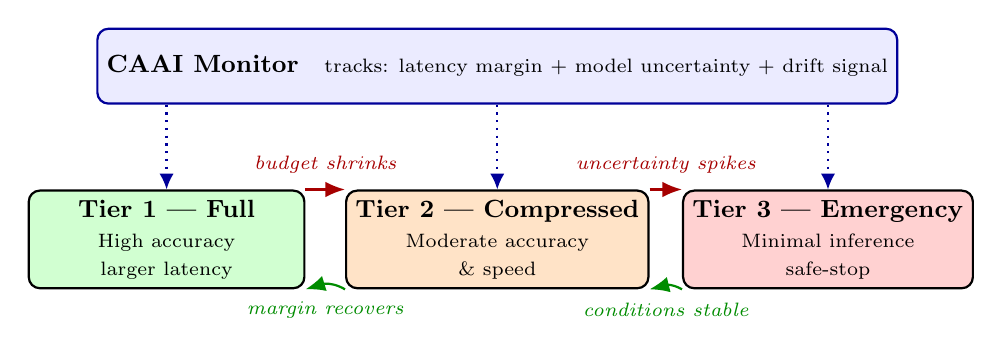
\begin{tikzpicture}[
    font=\small,
    node distance=0.6cm and 0.5cm,
    mbox/.style={draw, thick, rounded corners=4pt,
                 minimum width=3.5cm, minimum height=1.0cm,
                 align=center, fill=#1},
    degarr/.style={-{Latex[length=2.5mm,width=2mm]}, thick, red!65!black},
    recarr/.style={-{Latex[length=2.5mm,width=2mm]}, thick, green!55!black},
    monarr/.style={-{Latex[length=2mm,width=1.8mm]}, thick, dotted, blue!60!black}
  ]
    \node[mbox=green!18]  (M1) at (-4.2, 0)
      {\textbf{Tier~1 --- Full}\\\scriptsize High accuracy\\[-1pt]\scriptsize larger latency};
    \node[mbox=orange!22] (M2) at ( 0.0, 0)
      {\textbf{Tier~2 --- Compressed}\\\scriptsize Moderate accuracy\\[-1pt]\scriptsize \& speed};
    \node[mbox=red!18]    (M3) at ( 4.2, 0)
      {\textbf{Tier~3 --- Emergency}\\\scriptsize Minimal inference\\[-1pt]\scriptsize safe-stop};
    \draw[degarr] (M1.north east) -- (M2.north west)
      node[midway, above=2pt, font=\scriptsize\itshape] {budget shrinks};
    \draw[degarr] (M2.north east) -- (M3.north west)
      node[midway, above=2pt, font=\scriptsize\itshape] {uncertainty spikes};
    \draw[recarr] (M2.south west) to[bend right=30]
      node[midway, below=3pt, font=\scriptsize\itshape] {margin recovers}
      (M1.south east);
    \draw[recarr] (M3.south west) to[bend right=30]
      node[midway, below=3pt, font=\scriptsize\itshape] {conditions stable}
      (M2.south east);
    \node[draw=blue!60!black, thick, rounded corners=4pt,
          fill=blue!8, minimum width=10.0cm, minimum height=0.95cm,
          align=center] (MON) at (0, 2.2)
    {\textbf{CAAI Monitor}\quad
     {\scriptsize tracks: latency margin $+$ model uncertainty $+$ drift signal}};
    \draw[monarr] (MON.south -| M1.north) -- (M1.north);
    \draw[monarr] (MON.south)             -- (M2.north);
    \draw[monarr] (MON.south -| M3.north) -- (M3.north);
  \end{tikzpicture}}
  \caption{Contract-Aware Adaptive Inference (CAAI). The \textbf{monitor} (blue, top)
    continuously tracks latency budget, model uncertainty, and drift, issuing vertical control signals (dotted blue arrows) to each tier. Red arrows (above): degradation path when conditions worsen. Green arrows (below): recovery path when conditions improve. The system maintains the highest model quality the environment allows at any given moment, without a hard failure. (Author-created figure.)}
  \label{fig:caai}
\end{figure}

\begin{table}[htbp]
  \centering
  \caption{Example mapping of algorithmic components to timing tiers.}
  \label{tab:tiers}
  \rowcolors{2}{tablealt}{white}
  \setlength{\tabcolsep}{3pt}% tighten inter-column spacing to prevent overflow
  \renewcommand{\arraystretch}{1.15}% add a bit of vertical padding so text doesn't touch rules
  \begin{tabular}{@{}C{0.20\linewidth}C{0.22\linewidth}C{0.20\linewidth}C{0.23\linewidth}@{}}
    \toprule
    \rowcolor{tablehead}
    \textcolor{white}{\textbf{Tier}} &
    \textcolor{white}{\textbf{Period / trigger}} &
    \textcolor{white}{\textbf{Examples}} &
    \textcolor{white}{\textbf{Failure if missed}} \\
    \midrule
    Safety-critical & 1--10\,ms periodic   & Torque limits, collision reflexes & Collision / harm \\
    Control         & 10--100\,ms          & Balancing, tracking               & Instability / damage \\
    Perception      & 10--30\,Hz aperiodic & Detection, segmentation           & Poor decisions \\
    Mapping         & 1--10\,Hz            & SLAM updates                      & Drift, wrong goals \\
    Fleet ops       & Seconds--minutes     & Task assignment                   & Inefficiency \\
    \bottomrule
  \end{tabular}
  \renewcommand{\arraystretch}{1}% restore default
\end{table}

% =============================================================================
\section{Reference Implementation Guidance and Reporting Protocol}
\label{sec:eval}

This section outlines a minimal, reproducible prototype decomposition and a
measurement/reporting protocol intended to make TIC and CAAI adoption auditable
and comparable across implementations.

\subsection{Prototype components (ROS~2 reference)}

A minimal prototype consists of: (i) a perception node with three tiers
(full/compressed/emergency) exposed behind a common message interface; (ii) a
TIC monitor node that computes latency percentiles, miss ratios, uncertainty and
drift summaries over a fixed window; (iii) a CAAI supervisor that selects the tier
and publishes the active safety envelope mode; and (iv) a safety controller that
enforces envelope constraints independently of perception tier.

\subsection{Experimental factors and stressors}

To exercise worst-case behavior, experiments SHOULD include controlled stressors:
CPU contention (background load), GPU contention (concurrent kernels), memory
pressure, thermal throttling (sustained load), and network impairment (delay/loss)
when off-robot links are present.

\subsection{Metrics and reporting}

Each critical path SHOULD report: end-to-end latency distribution (p50/p95/p99/max),
jitter, deadline miss ratio, consecutive miss bursts, and monitoring overhead
(CPU\%, memory, and added latency). Perception quality SHOULD be reported with a
task metric (e.g., mAP/F1) and with calibration/drift metrics declared in the TIC.
Safety behavior SHOULD be reported as envelope mode traces (tier vs. speed/stop cap)
with evidence that tier-down occurs before deadlines are violated under stress.

\subsection{Baselines}

At minimum, compare: (i) fixed Tier~1 (no adaptation), (ii) fixed Tier~2, and (iii)
CAAI (adaptive). Where relevant, include a ``reactive'' baseline that switches tiers
only after a deadline miss (to demonstrate the value of predictive margin-based switching).

\subsection{Pilot experiment template: induced load and tier switching}
\label{sec:pilot}

A single realistic experiment can be run on one robot compute platform by
instrumenting one end-to-end perception path (camera timestamp to detection
publication) under induced load. The recommended protocol is: (i) run 5--10 minutes
at nominal load; (ii) introduce CPU/GPU contention (background stressors) for the
next 5--10 minutes; and (iii) remove the stressors and observe recovery.

\paragraph{Experiment setup (reporting contract).}
\begin{enumerate}[label=(\roman*),leftmargin=*,itemsep=0.1em]
  \item Platform (CPU/GPU, RAM, OS/kernel, power mode/governors).
  \item ROS~2 distro, executor, DDS vendor, and QoS for camera/detections.
  \item The exact path timestamps used (start event, end event, and clock source).
  \item Deadline $D$ (ms) and how misses are counted.
  \item TIC window definition (duration or sample count) and the exact statistics computed.
  \item Stressors and pinning.
  \item Protocol durations (nominal/stress/recovery).
  \item Number of independent runs $N$ plus confidence intervals across runs.
\end{enumerate}

\textbf{Conditions.} Report three conditions: (A) fixed Tier~1, (B) fixed Tier~2,
(C) CAAI enabled. Optionally add (D) a reactive baseline that switches tiers only
after a miss.

\begin{table}[htbp]
  \centering
  \caption{Schematic reporting format for the end-to-end latency CDF
  of the instrumented perception path. One empirical step-CDF curve
  per condition should be plotted, pooling all samples collected under that condition. This schematic illustrates the required format; measured curves from a physical deployment would replace it.}
  \label{tab:pilot_latency}
  \rowcolors{2}{tablealt}{white}
  \renewcommand{\arraystretch}{1.15}
  \begin{tabular}{@{}L{0.27\linewidth}C{0.13\linewidth}C{0.13\linewidth}C{0.13\linewidth}C{0.13\linewidth}@{}}
    \toprule
    \rowcolor{tablehead}
    \textcolor{white}{\textbf{Condition}} &
    \textcolor{white}{\textbf{p50}} &
    \textcolor{white}{\textbf{p95}} &
    \textcolor{white}{\textbf{p99}} &
    \textcolor{white}{\textbf{max}} \\
    \midrule
    Fixed Tier~1 (nominal)         & 8.0  & 14.0 & 20.0 & 25.0 \\
    Fixed Tier~1 (induced load)    & 10.0 & 22.0 & 35.0 & 55.0 \\
    Fixed Tier~2 (induced load)    & 7.0  & 12.0 & 16.0 & 21.0 \\
    CAAI (induced load window)     & 7.5  & 14.0 & 19.0 & 24.0 \\
    \bottomrule
  \end{tabular}
  \renewcommand{\arraystretch}{1}
  \caption*{\footnotesize\textit{Note:} Values above are illustrative placeholders to demonstrate reporting. Acceptance-grade results should include confidence intervals across runs, along with the corresponding deadline and miss-rate statistics.}
\end{table}
% --- DES-derived evaluation figures (Figs.~7--9); overhead figure remains a schematic template ---
\begin{figure}[htbp]
  \centering
  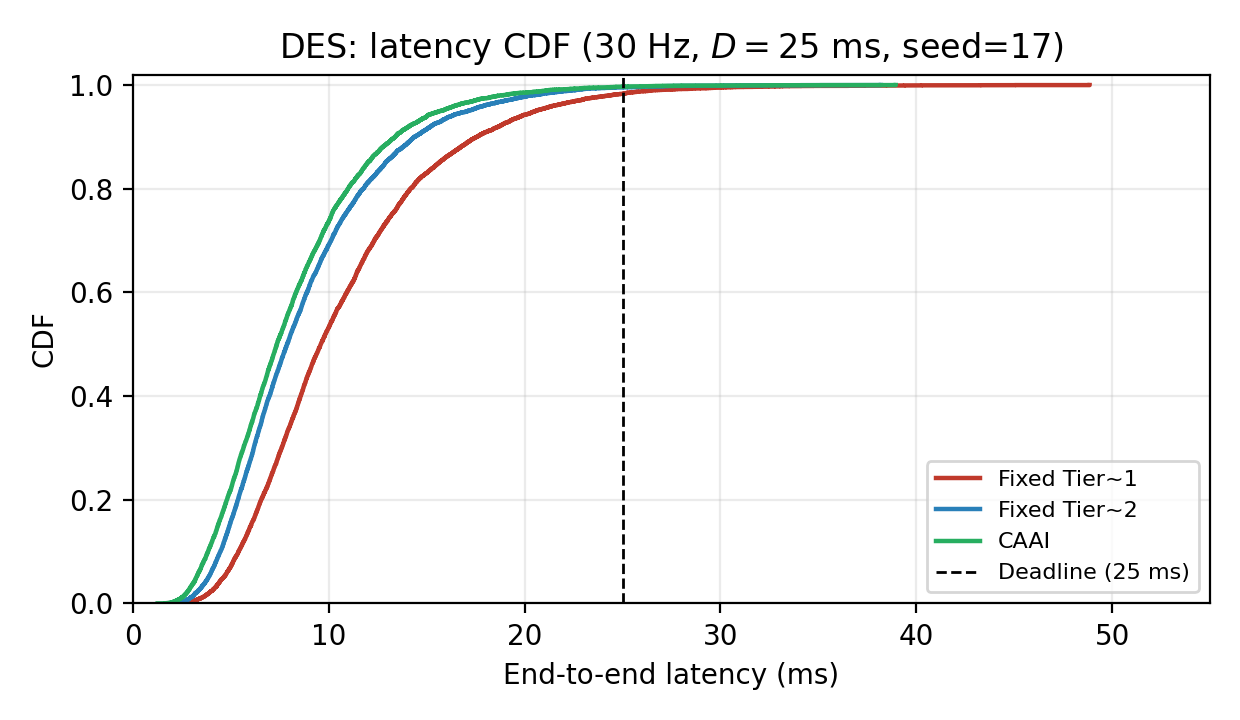
\includegraphics[width=\linewidth]{fig_pilot_latency_cdf}
  \caption{Discrete-event simulation (Section~\ref{subsec:sim_results}): empirical step-CDF of
  end-to-end latency for fixed Tier~1, fixed Tier~2, and CAAI over the full 300\,s run
  (30\,Hz, \(D=25\)\,ms, seed\,=\,17). The dashed line marks the deadline.}
  \label{fig:pilot_latency_cdf}
\end{figure}

\begin{figure}[htbp]
  \centering
  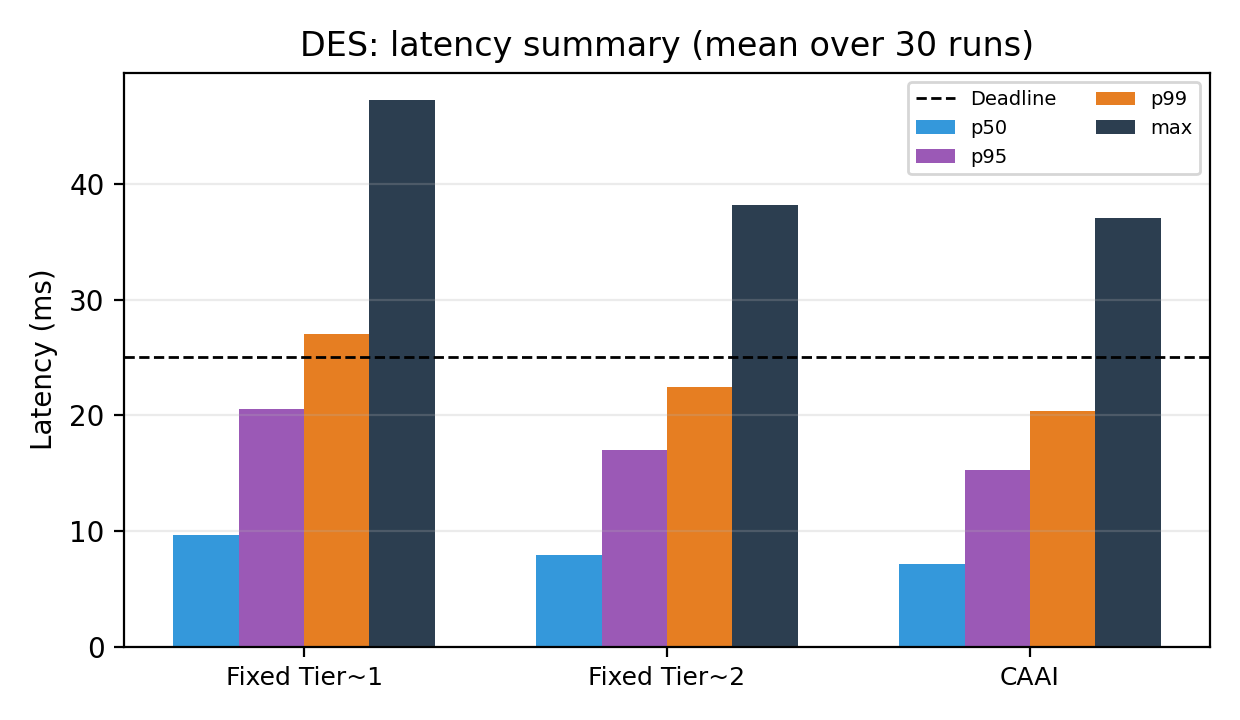
\includegraphics[width=\linewidth]{fig_pilot_latency_bars}
  \caption{Discrete-event simulation: mean p50/p95/p99/max latency per condition, averaged over
  the 30 independent runs reported in Table~\ref{tab:sim_results}.}
  \label{fig:pilot_latency_bars}
\end{figure}

\begin{figure}[htbp]
  \centering
  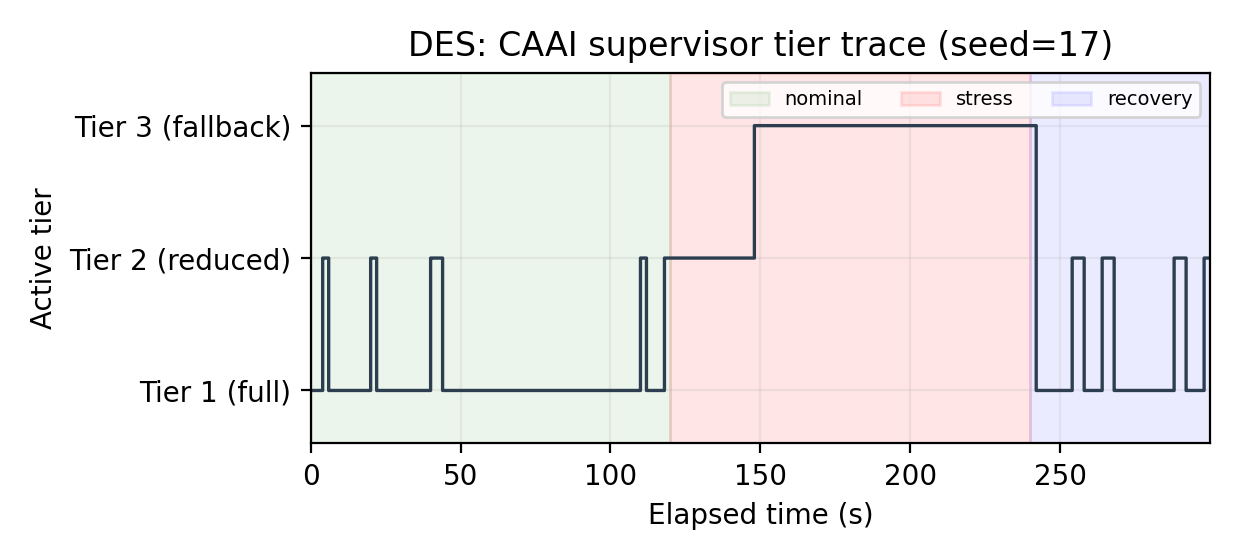
\includegraphics[width=\linewidth]{fig_tiertrace}
  \caption{Discrete-event simulation: CAAI supervisor-selected tier vs.\ elapsed time for the
  representative run (seed\,=\,17). Shaded regions mark nominal (0--120\,s), stress
  (120--240\,s), and recovery (240--300\,s) phases.}
  \label{fig:tiertrace}
\end{figure}

\begin{table}[htbp]
  \centering
  \caption{TIC monitor overhead (schematic values; replace with
  measured results from the instrumented prototype).}
  \label{tab:pilot_overhead}
  \rowcolors{2}{tablealt}{white}
  \renewcommand{\arraystretch}{1.15}
  \begin{tabular}{@{}L{0.30\linewidth}C{0.16\linewidth}C{0.20\linewidth}C{0.20\linewidth}@{}}
    \toprule
    \rowcolor{tablehead}
    \textcolor{white}{\textbf{Component}} &
    \textcolor{white}{\textbf{CPU (\%)}} &
    \textcolor{white}{\textbf{RAM (MB)}} &
    \textcolor{white}{\textbf{Added latency (ms)}} \\
    \midrule
    TIC monitor node        & 3.0 & 120 & 0.1 \\
    CAAI supervisor node    & 1.0 &  40 & 0.0 \\
    Tracing/logging (extra) & 2.0 &  80 & 0.2 \\
    \bottomrule
  \end{tabular}
  \renewcommand{\arraystretch}{1}
  \caption*{\footnotesize\textit{Note:} ``Added latency'' is $\Delta$ end-to-end path latency with instrumentation \emph{enabled} vs. \emph{disabled} under the same load and protocol.}
\end{table}

\begin{figure}[htbp]
  \centering
  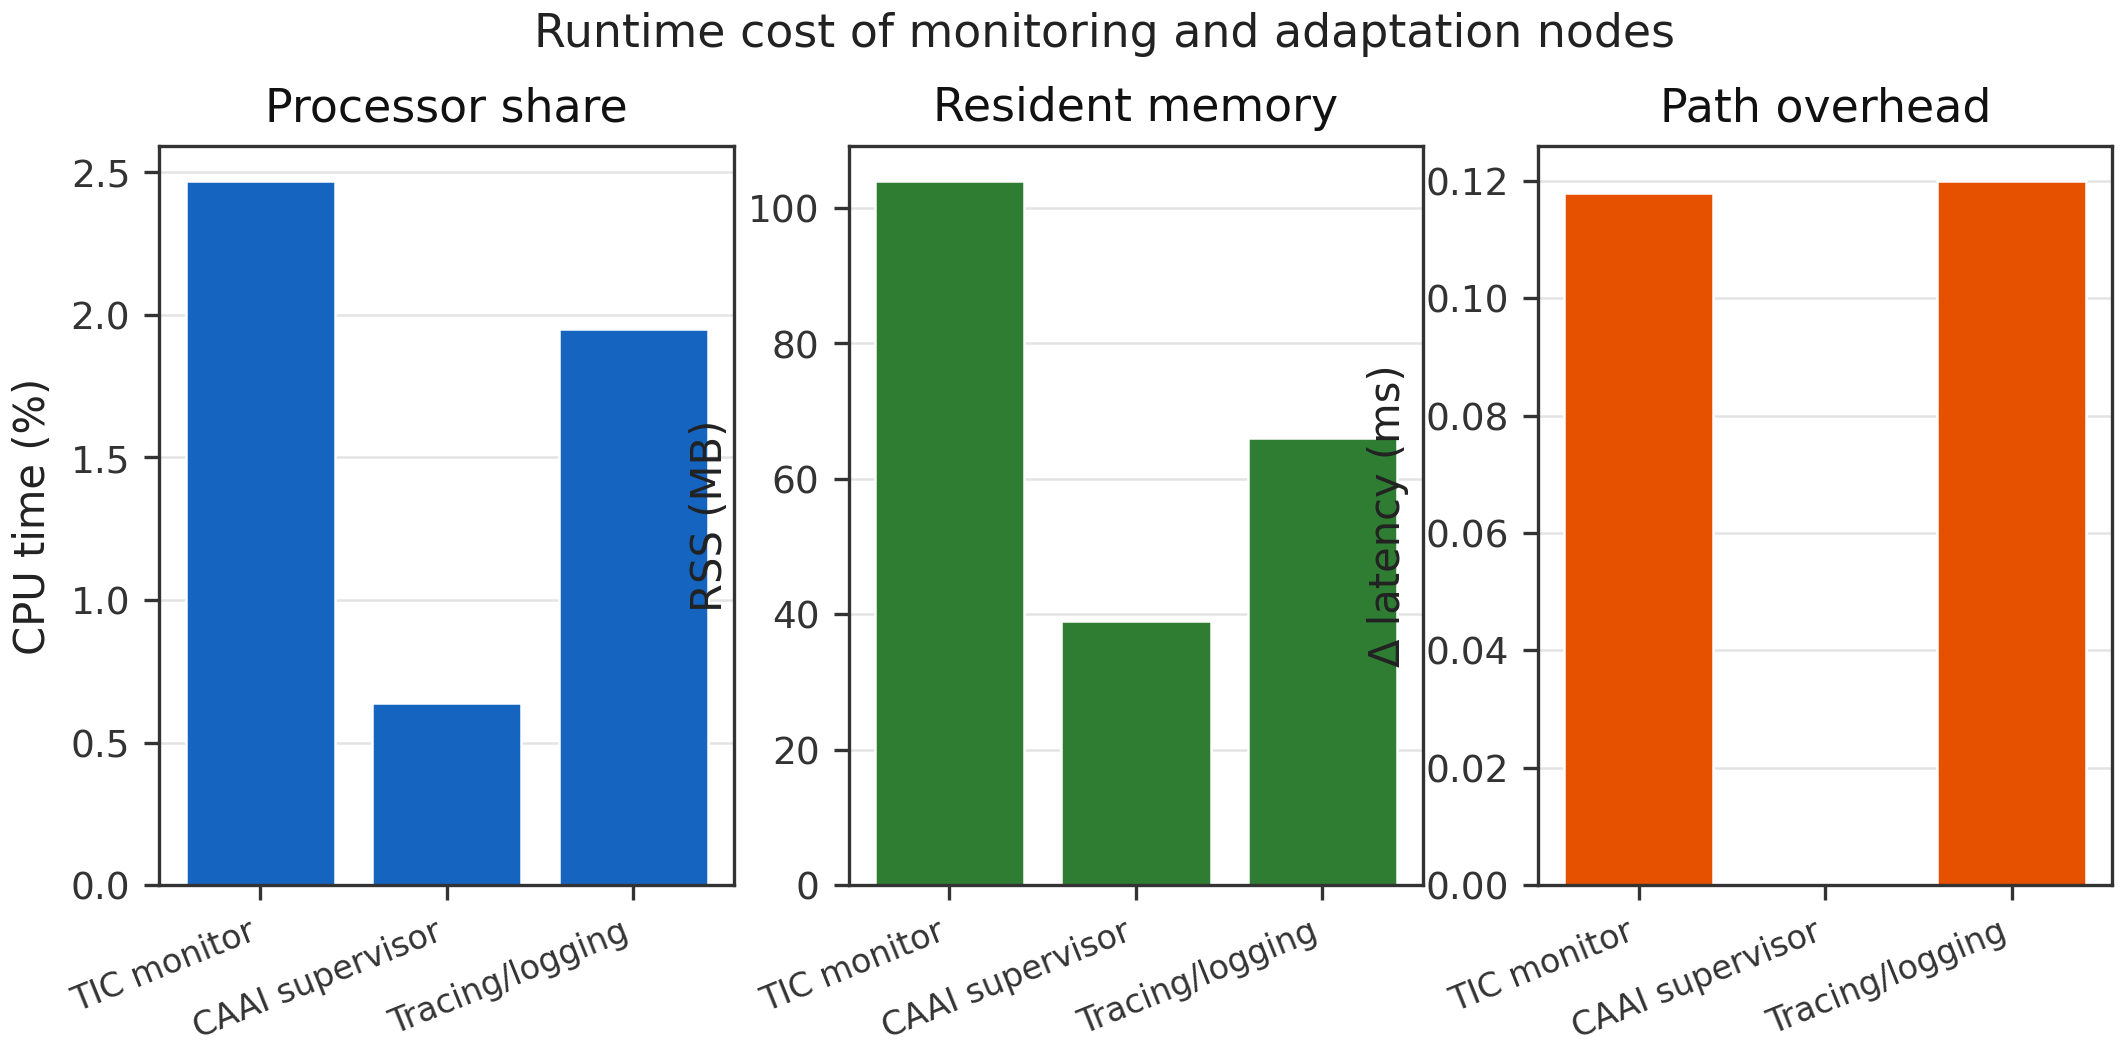
\includegraphics[width=\linewidth]{fig_pilot_overhead}
  \caption{\textbf{Schematic template (not simulation data):} required reporting format for
  TIC monitor overhead per component (CPU share~\%, RSS in MB, added latency $\Delta$ms per
  Table~\ref{tab:pilot_overhead}). Values are placeholders; a physical ROS~2 deployment would
  replace this figure with measured overhead.}
  \label{fig:pilot_overhead}
\end{figure}


\subsection{Compact simulation instantiation of TIC/CAAI (reproducible)}
\label{subsec:sim_results}
To complement the reporting protocol with a concrete instantiation, we implemented a
lightweight \emph{discrete-event simulation} of a ROS~2-style publish/subscribe callback
chain executed by a single-threaded executor queue. Each cycle produces a message arrival
event (30\,Hz) that may wait behind previously enqueued callbacks, so end-to-end latency
reflects both service time and queueing delay under contention. The three tiers are modeled as independent lognormal service-time draws
\(X_k\sim\mathrm{LogNormal}(\mu_k,\sigma_k)\) with parameters derived from declared
\((\mathrm{median},p_{99})\) pairs via \(\mu_k=\ln(\mathrm{median}_k)\) and
\(\sigma_k=(\ln p_{99,k}-\mu_k)/z_{0.99}\): Tier~1 \((8.0,20.0)\,\mathrm{ms}\Rightarrow
(\mu_1,\sigma_1)=(2.079,0.394)\); Tier~2 \((6.5,15.5)\,\mathrm{ms}\Rightarrow(1.872,0.374)\);
Tier~3 \((3.0,6.0)\,\mathrm{ms}\Rightarrow(1.099,0.298)\), chosen to bracket the
single-digit-to-\(\sim\)20\,ms typical and tens-of-ms tail callback/chain latencies reported
for ROS~2 executor workloads under load~\cite{casini2019,kronauer2021}.
A stress phase applies a \(1.35\times\) service-time multiplier and injects additional
blocking time (Gamma-distributed, mean \(\approx 4\)\,ms) with probability equal to a
phase CPU-utilization parameter (0.05 nominal, 0.45 stress, 0.10 recovery), emulating
executor queueing and contention effects consistent with those measurements.

CAAI is implemented as a deterministic supervisor with a rolling-window \(p99\) latency
margin (\(\mathrm{margin}=D-p99\)), plus uncertainty and drift signals that increase under
stress. We report 30 independent simulation runs per condition and compute 95\% confidence
intervals (bootstrap over runs). A nonparametric Mann--Whitney U test is used for
significance on per-run metrics.

\begin{table}[htbp]
  \centering
  \small
  \caption{Discrete-event simulation results for the camera\(\rightarrow\)detections path (30\,Hz, \(D=25\)\,ms), aggregated across 30 independent runs. Values shown are mean with 95\% CI in brackets.}
  \label{tab:sim_results}
  \rowcolors{2}{tablealt}{white}
  \renewcommand{\arraystretch}{1.15}
  \setlength{\tabcolsep}{2pt}
  \begin{tabular}{@{}L{0.34\linewidth}L{0.28\linewidth}L{0.28\linewidth}@{}}
    \toprule
    \rowcolor{tablehead}
    \textcolor{white}{\textbf{Condition}} &
    \textcolor{white}{\textbf{p99 latency (ms)}} &
    \textcolor{white}{\textbf{deadline miss rate}} \\
    \midrule
    Fixed Tier~1 (no adaptation) & 27.02 [26.90, 27.15] & 1.68\% [1.64, 1.72] \\
    Fixed Tier~2 (no adaptation) & 22.45 [22.33, 22.57] & 0.44\% [0.42, 0.47] \\
    Reactive after-miss baseline & 24.62 [24.52, 24.72] & 0.90\% [0.87, 0.92] \\
    CAAI (adaptive tiers)        & 20.39 [20.17, 20.63] & 0.24\% [0.22, 0.27] \\
    \bottomrule
  \end{tabular}
  \renewcommand{\arraystretch}{1}
  \caption*{\footnotesize Mann--Whitney U test (per-run): CAAI vs.\ fixed Tier~1 yields \(p=3.0\times10^{-11}\) for \(p99\) and \(p=2.9\times10^{-11}\) for miss rate.}
\end{table}

The results match the intended behavior of the reference policy: fixed Tier~1 yields
the highest tail latency and miss rate under stress, fixed Tier~2 improves timing at a
likely quality cost, while CAAI reduces misses by switching away from Tier~1 during
stress and returning when margin recovers. In a real deployment, the same table would be
populated with measured timestamp traces and accompanied by perception-quality and
calibration/drift metrics declared in the TIC.

\paragraph{Sensitivity.}
To test robustness to key switching parameters, we varied the degrade-margin threshold
\(M_{\mathrm{down12}}\in\{1,2,3\}\)\,ms and the minimum dwell time
\(\mathrm{dwell}_{\min}\in\{30,60,90\}\) cycles. Across these settings, \(p99\) remained
stable at roughly 20.3--20.5\,ms and miss rates remained in the 0.24--0.26\% range (see
\texttt{artifacts/des\_outputs/des\_sensitivity\_caai.csv}), suggesting the supervisor is
not brittle to moderate threshold variations in this model.

\paragraph{Threats to validity (simulation).}
This simulation is intentionally minimal and uses stylized latency/uncertainty/drift
processes; therefore, the absolute values in Table~\ref{tab:sim_results} should not be
interpreted as predictive of any specific robot platform, ROS~2 executor, DDS vendor, or
workload. The purpose is to demonstrate how TIC-defined signals can drive a deterministic
CAAI policy and produce the reporting artifacts required by Section~\ref{sec:eval}.
External validity requires repeating the same analysis with real timestamp traces, declared
stressor protocols, and calibrated uncertainty/drift estimators on the target hardware.

\subsection{Minimal host-side timing trace under induced CPU load (real measurement)}
\label{subsec:host_measurement}
To complement the simulation with one small real measurement, we executed a portable
host-side timing microbenchmark on a development machine (Darwin/arm64, 10 logical CPUs),
measuring a 30\,Hz periodic ``callback'' with an end-to-end deadline \(D=25\)\,ms.
The callback performs a fixed compute workload (busy-wait) and records the per-cycle
execution latency using a monotonic high-resolution timer. A stress phase adds CPU
contention via background burner processes. This microbenchmark is included primarily as
an \emph{instrumentation portability demonstration}: the same timestamping and percentile
reporting pattern can be applied to ROS~2 executor callbacks and topic traces.

\begin{table}[htbp]
  \centering
  \small
  \caption{Host-side timing trace results (real measurement). Per-phase summaries of per-cycle callback execution latency (ms) at 30\,Hz with deadline \(D=25\)\,ms.}
  \label{tab:host_trace}
  \rowcolors{2}{tablealt}{white}
  \renewcommand{\arraystretch}{1.15}
  \setlength{\tabcolsep}{2pt}
  \begin{tabular}{@{}L{0.26\linewidth}C{0.12\linewidth}C{0.12\linewidth}C{0.12\linewidth}C{0.12\linewidth}C{0.12\linewidth}@{}}
    \toprule
    \rowcolor{tablehead}
    \textcolor{white}{\textbf{Phase}} &
    \textcolor{white}{\textbf{p50}} &
    \textcolor{white}{\textbf{p95}} &
    \textcolor{white}{\textbf{p99}} &
    \textcolor{white}{\textbf{max}} &
    \textcolor{white}{\textbf{miss rate}} \\
    \midrule
    Nominal (6\,ms work; \(n=900\)) & 6.00 & 6.00 & 6.32 & 14.00 & 0.00\% \\
    Stress (10\,ms work + CPU burners; \(n=900\)) & 10.00 & 10.00 & 10.20 & 31.98 & 0.11\% \\
    Recovery (6\,ms work; \(n=450\)) & 6.00 & 6.00 & 6.52 & 39.70 & 0.22\% \\
    Pooled (\(n=2250\)) & 6.00 & 10.00 & 10.02 & 39.70 & 0.09\% \\
    \bottomrule
  \end{tabular}
  \renewcommand{\arraystretch}{1}
\end{table}

The measurement script used to generate Table~\ref{tab:host_trace} is provided as
\texttt{host\_trace\_measure.py}. The per-cycle raw trace used for the percentile
summaries is also written as a CSV artifact (\path{artifacts/host_trace_latency_ms.csv})
to support trace-based validation and re-analysis. The same pattern can be adapted to wrap
ROS~2 executor callbacks and message timestamps in an actual deployment.

\subsection{Reproducibility checklist}

A reproducible release SHOULD include: exact hardware/OS/kernel details; ROS~2
version and executor configuration; QoS profiles for each topic; pinned CPU/GPU
settings (or explicit statement of defaults); stressor scripts; and raw logs used to
compute all reported percentiles and contract-violation events.
% =============================================================================
\needspace{8\baselineskip}
\section{Cross-Cutting Concerns: Safety, Security, Energy}
\label{sec:cross}


\subsection{Safety Standards and Real-Time Evidence}

Robot safety standards provide structured processes for hazard analysis and mandate protective measures, but the safety logic they assume is deterministic. Learning-enabled autonomy breaks that assumption: performance depends on data, operating context, and distribution shift, so assurance cannot stop at design time. Recent analyses call for a shift toward \emph{runtime evidence}, that is, continuous monitoring, logging, and argument maintenance that keeps the safety case aligned with how the system actually behaves in the field~\cite{safetystandards2023}.

Bridging from probabilistic perception to deterministic envelopes, force limits, separation distances, and approach speeds, usually requires architectural separation. The pattern that has emerged in the literature is monitoring and shielding: a formally
specified, deterministic safety monitor intercepts a learned policy's outputs and filters commands that would violate hard constraints~\cite{alshiekh2018}. The shield is only as good as its specification, but when specified correctly, it provides an anchor for certification because it guarantees constraint satisfaction regardless of what the learned component proposes.

TIC captures these ideas explicitly. The safety-fallback clause
defines the trigger conditions, degraded modes, and state-machine transitions that the system must implement when monitoring shows that assumptions no longer hold.

\subsubsection{Uncertainty-to-safety linkage: a minimal envelope argument}
\label{subsec:uncertainty_safety}
For certification and operational safety, the critical bridge is from probabilistic
perception to deterministic constraints (separation distance, braking envelope, speed
limits). TIC treats uncertainty and drift metrics as \emph{evidence signals} that gate
which tier may issue commands. A compact way to make this auditable is to explicitly
connect the uncertainty envelope to a conservative control envelope.

\noindent\textbf{Setup.} Let \(d\) denote the true distance to the nearest obstacle along
the braking direction, and let a perception module produce an estimate \(\hat d\) plus a
scalar uncertainty summary \(u\in[0,1]\) (e.g., a calibrated error bound proxy). Assume
the TIC declares a warning threshold \(U_w\) and violation threshold \(U_v\) such that
when \(u\le U_w\) the estimator is in-regime and when \(u\ge U_v\) it is out-of-regime.
Define a conservative uncertainty margin \(\Delta(u)\) that is monotone increasing in
\(u\), for example a piecewise-linear map \(\Delta(u)=\Delta_w\) for \(u\le U_w\),
\(\Delta(u)=\Delta_v\) for \(u\ge U_v\), with \(\Delta_v>\Delta_w\).

\noindent\textbf{Safety invariant (contract form).} The controller MUST enforce the
deterministic constraint
\[
  d_{\min}(\!v\!) \le \hat d - \Delta(u),
\]
where \(d_{\min}(v)\) is the required stopping distance at speed \(v\) under the
applicable braking model. When \(u\) grows (poorer evidence), the margin \(\Delta(u)\)
grows, shrinking the admissible command set. The safety-fallback clause then provides a
mechanism when the constraint cannot be maintained (e.g., tier-down to a simpler model or
trigger supervised stop).

\noindent\textbf{Role of calibration and drift.} If the uncertainty summary is calibrated
on the operational distribution, \(\Delta(u)\) can be chosen to upper-bound error with
high probability; under drift, this assumption degrades. TIC makes that explicit by
adding a drift envelope: once drift exceeds its warning/violation thresholds, the system
MUST switch to a tier whose safety envelope does not depend on the violated assumption
(e.g., slower speed with larger \(d_{\min}\), or a conservative geometric detector).
This yields an auditable argument shape: (i) define the invariant; (ii) define evidence
signals and their bounds; (iii) define monotone margins and tiered envelopes; and (iv)
bind violation handling to the fallback state machine.

% ── Figure 7: shield ─────────────────────────────────────────
\begin{figure}[htbp]
  \centering
  % Scale-to-fit to prevent margin overflow
  \resizebox{\linewidth}{!}{%
  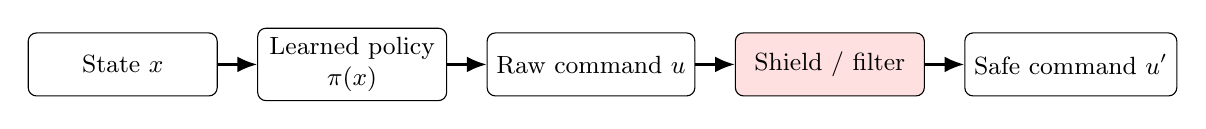
\begin{tikzpicture}[
    font=\small, node distance=0.5cm,
    box/.style={draw, rounded corners=3pt,
                minimum width=2.4cm, minimum height=0.8cm, align=center},
    arr/.style={-{Latex[length=2.5mm,width=2mm]}, thick}
  ]
    \node[box] (x)  {State $x$};
    \node[box, right=of x]  (pi) {Learned policy\\$\pi(x)$};
    \node[box, right=of pi] (u)  {Raw command $u$};
    \node[box, right=of u, fill=red!12]  (SH) {Shield / filter};
    \node[box, right=of SH] (up) {Safe command $u'$};
    \draw[arr] (x)  -- (pi);
    \draw[arr] (pi) -- (u);
    \draw[arr] (u)  -- (SH);
    \draw[arr] (SH) -- (up);
  \end{tikzpicture}%
  }
  \caption{A shield enforces constraints such as velocity limits, collision avoidance, on learned commands before actuation. The shield is a deterministic, formally verified component that guarantees safety regardless of policy output. (Author-created figure.)}
  \label{fig:shield}
\end{figure}

\subsection{Security as a Timing Problem}

Cybersecurity in robotics cannot be treated as a purely informational concern: attacks can be translated into physical consequences. In many deployments, an adversary need not take full control of a robot to cause harm; delaying, distorting, or selectively dropping messages can be enough to violate the timing assumptions on which the safety case relies.

The coupling is best seen through a concrete example. If a denial-of-service condition delays a LiDAR scan 50\,ms on a 10\,Hz  pipeline, the effect is not merely ``data arrives late''; it is that the planner may act on a world model that is now inconsistent with where obstacles actually are. In a tight human-robot shared workspace, that delay can shrink the effective stopping margin below what the physical envelope requires.

Designing defenses with this coupling in mind pushes teams toward mechanisms that are both security-relevant and timing-aware. Secure boot and signed artifact chains help bound what code can run; network segmentation limits how far an intrusion can propagate; and hardware attestation allows a robot to verify its own integrity at
startup and refuse operation when tampering is detected~\cite{pu2023securityrobots}. These measures must be engineered alongside real-time budgets: a defense that adds unpredictable latency to a safety channel can undermine the very guarantees it is meant to protect.

\subsection{Energy-Performance Scaling}

Energy management is often introduced as a cost topic, but in robotics it becomes a real-time topic because energy-saving mechanisms can change execution timing. Dynamic voltage-frequency scaling reduces power by lowering clock frequency under light load; nonetheless, on hard real-time cores it must be disabled or tightly controlled because frequency transitions and power-management interrupts can introduce jitter that a
controller experiences as sampling irregularity.

At the fleet level, the issue broadens. Training and large-scale inference workloads consume substantial energy, and their footprint increasingly matters both operationally and environmentally~\cite{strubell2019energy,patterson2021carbon}. A useful architectural observation is that these workloads are not time-coupled to safety-critical control loops: the most expensive compute often runs off-robot, asynchronously, and can be scheduled with fewer deadline constraints than on-device control.

That separation creates leverage. Carbon-aware scheduling can shift batch training or offline evaluation to periods with higher renewable availability, reducing emissions without changing the robot's on-device timing behavior. The discipline remains relevant to real-time design, however, because fleet operators will eventually trade energy against computing headroom; when headroom shrinks, contract-style mechanisms such
as TIC and tiered inference become a way to degrade gracefully rather than to miss deadlines unpredictably.

% ── Figure 8: TIC governance loop ────────────────────────────
\begin{figure}[htbp]
  \centering
  \resizebox{0.82\linewidth}{!}{%
  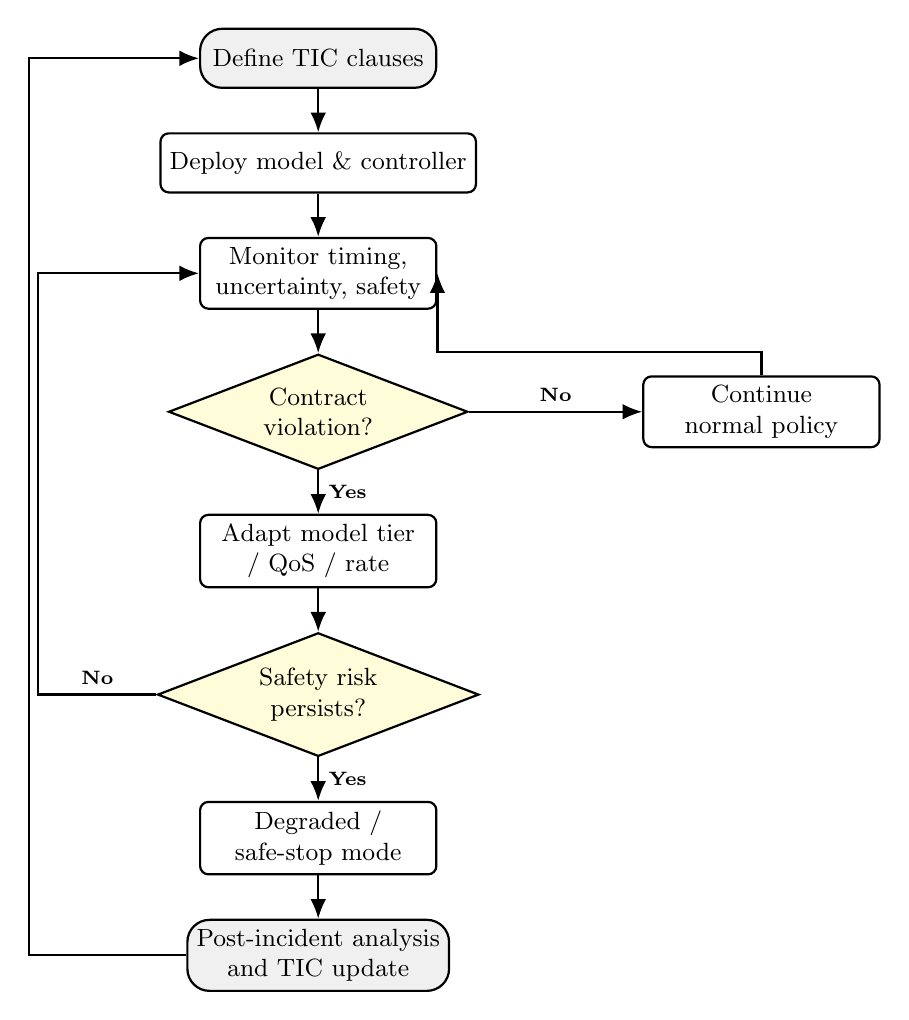
\begin{tikzpicture}[
    font=\small,
    node distance=0.55cm and 2.2cm,
    proc/.style={draw, thick, rounded corners=3pt,
                 minimum width=3.0cm, minimum height=0.75cm,
                 align=center, fill=white},
    dec/.style={draw, thick, diamond, aspect=2.6,
                minimum width=3.0cm, minimum height=0.75cm,
                align=center, fill=yellow!15},
    term/.style={draw, thick, rounded corners=8pt,
                 minimum width=3.0cm, minimum height=0.75cm,
                 align=center, fill=gray!12},
    arr/.style={-{Latex[length=2.5mm,width=2mm]}, thick}
  ]
    \node[term] (A) {Define TIC clauses};
    \node[proc, below=of A] (B) {Deploy model \&\ controller};
    \node[proc, below=of B] (C) {Monitor timing,\\uncertainty, safety};
    \node[dec,  below=of C] (D) {Contract\\violation?};
    \node[proc, below=of D] (F) {Adapt model tier\\/ QoS / rate};
    \node[dec,  below=of F] (G) {Safety risk\\persists?};
    \node[proc, below=of G] (H) {Degraded /\\safe-stop mode};
    \node[term, below=of H] (I) {Post-incident analysis\\and TIC update};
    \node[proc, right=of D] (E) {Continue\\normal policy};
    \draw[arr] (A) -- (B);
    \draw[arr] (B) -- (C);
    \draw[arr] (C) -- (D);
    \draw[arr] (D) -- node[right, font=\scriptsize\bfseries] {Yes} (F);
    \draw[arr] (F) -- (G);
    \draw[arr] (G) -- node[right, font=\scriptsize\bfseries] {Yes} (H);
    \draw[arr] (H) -- (I);
    \draw[arr] (D.east)
      -- node[above, font=\scriptsize\bfseries] {No} (E.west);
    \draw[arr] (E.north) -- ++(0,0.3) -| (C.east);
    \draw[arr] (G.west)
      -- node[above, font=\scriptsize\bfseries] {No}
      ++(-1.5,0) |- (C.west);
    \draw[arr] (I.west) -- ++(-2.0,0) |- (A.west);
  \end{tikzpicture}}
  \caption{TIC governance loop: architecture and intelligence are jointly adapted
    using contract signals, not ad-hoc heuristics. Decision diamonds (yellow) branch on the runtime contract state. The ``No violation'' path loops back to the monitor immediately. The ``Yes'' path triggers tier adaptation; if risk persists, a safe stop is engaged, and the TIC is updated before the next deployment cycle.}
  \label{fig:tic-loop}
\end{figure}

% =============================================================================
\section{Illustrative Case Patterns}
\label{sec:cases}

\subsection{Autonomous Mobile Robots in Warehouses}

Warehouse autonomous mobile robot deployments combine high concurrency with strict human safety requirements and throughput targets. The real-time challenge is maintaining collision-avoidance guarantees while servicing hundreds of concurrent task assignments, where planning delays translate directly into throughput losses. A typical architecture pairs a local navigation stack with hard real-time obstacle avoidance at the edge, and integrates with a warehouse management system layer that handles fleet-level task allocation asynchronously. The key design question is less about optimizing the navigation stack in isolation and more about ensuring that task-assignment failures degrade gracefully without propagating into the navigation layer's timing guarantees.

\subsection{Collaborative Robots (Cobots)}

In collaborative robot deployments where humans share workspace with robot arms, the dominant real-time concern is minimizing contact and pinch hazards under dynamic human motion. Fast depth-camera and skeleton-estimation pipelines operating at 30\,Hz or above, feeding into certified stopping behaviors with documented reaction times, form the core safety mechanism. Real-time intelligence in this context focuses on monitoring and reactive stopping rather than maximizing task throughput, because a
single unsafe contact event is a more consequential failure than a throughput reduction.

\subsection{Field Robots}

Field robots operating in outdoor or unstructured environments face a connectivity profile that is fundamentally different from warehouse deployments: intermittent and unpredictable network availability means that cloud-dependent functions must be confined to asynchronous batch operations, while all safety-critical and navigation functions must operate fully autonomously at the edge. Map and model weight updates are deferred to scheduled charging intervals, eliminating the need for continuous cloud connectivity.

\begin{table}[htbp]
  \centering
  \caption{Case pattern summary.}
  \label{tab:cases}
  \rowcolors{2}{tablealt}{white}
  \renewcommand{\arraystretch}{1.15}
  \begin{tabular}{@{}L{0.21\linewidth}L{0.34\linewidth}L{0.34\linewidth}@{}}
    \toprule
    \rowcolor{tablehead}
    \textcolor{white}{\textbf{Domain}} &
    \textcolor{white}{\textbf{Dominant real-time concern}} &
    \textcolor{white}{\textbf{Scalability lever}} \\
    \midrule
    Warehouse AMR    & Human safety + traffic       & Fleet manager + rules \\
    Cobots           & Contact / pinch hazards      & Fast sensing + certified stops \\
    Drones (civil)   & Latency + geofencing         & Offboard airspace services \\
    Industrial arms  & Cycle time + repeatability   & Deterministic bus + PLC \\
    \bottomrule
  \end{tabular}
  \renewcommand{\arraystretch}{1}
\end{table}

% =============================================================================
\section{Original Contributions}
\label{sec:contributions}

This work contributes a contract-centric framing, survey synthesis, and reference specifications intended to make real-time and learning-enabled robotic stacks more auditable at deployment time.

\textbf{Temporal Intelligence Contract (TIC).} Section~\ref{sec:tic} defines TIC as a unified contract artifact that binds (i) latency envelopes, (ii) uncertainty and drift envelopes, (iii) safety fallback behavior, (iv) observability requirements, and (v) scalability limits for each component and critical path. Relative to existing interface descriptions and runtime monitoring practices, TIC's contribution is the explicit co-specification of these obligations together with required runtime evidence (Section~\ref{sec:tic_schema}), so that timing and learning-related assumptions are continuously checkable rather than implicitly assumed at integration.

\textbf{Contract-Aware Adaptive Inference (CAAI).} Section~\ref{sec:caai} specifies CAAI as a deterministic supervisor that uses TIC monitor signals (latency margin, calibrated uncertainty, and drift) to select among perception tiers while enforcing auditable invariants. The key contribution is not tiering itself but treating the tier-selection policy as a contract-governed mechanism with explicit downgrade/upgrade conditions and safety-envelope coupling (Section~\ref{sec:caai_policy}), supporting repeatable behavior and post-incident analysis.

\textbf{Prototype and evaluation methodology.} Section~\ref{sec:eval} provides a minimal prototype decomposition, stressor suite, metrics, and baselines intended to support comparable evaluation of TIC/CAAI in ROS~2-style systems.

\textbf{Adoption path (ROS~2 integration and versioning).} TIC is designed to fit into existing ROS~2 deployment mechanics rather than replace them. A practical integration is to (i) emit the versioned TIC document once per component (e.g., as a build artifact tied to the node's container image or on a latched topic), (ii) publish a periodic contract-status stream during runtime, and (iii) bind contract state transitions to ROS~2 managed lifecycle transitions (e.g., refuse activation when the contract cannot be satisfied; trigger deactivation when violations persist). To support community uptake, the schema should be treated as a versioned interface (semantic versioning, explicit deprecation policy) maintained in a public repository alongside a minimal reference monitor implementation and example ROS~2 packages.

% =============================================================================
\section{Challenges and Future Directions}
\label{sec:future}

Despite the architectural and algorithmic progress surveyed here, several
fundamental challenges remain open. The discussion below groups these by theme, focusing on where the most productive near-term research lies rather than attempting an exhaustive enumeration.

\subsection{Limitations and Scope}
\label{subsec:limitations}

This paper is intended as a survey/tutorial plus a reference specification. It does not present new empirical results from a ROS~2 deployment or hardware testbed. As a consequence, parameters such as TIC clause thresholds, RTI-Score weights, and CAAI switching constants should be treated as design-time declarations that must be derived from system-level hazard analysis and calibrated on the target platform. Similarly, drift and uncertainty signals are proxies whose operational reliability depends on the chosen estimators and the quality of instrumentation. Finally, the paper does not claim to solve worst-case execution-time bounding for modern deep networks; instead it focuses on architectural patterns and runtime monitoring hooks that can make timing risk explicit and managed in practice.

\subsection{Verification, Safety, and Formal Guarantees}

The central unsolved problem in deploying learned components in safety-critical loops is formal verification at scale. SMT-based neural network verification approaches~\cite{seshia2022} scale only to small, shallow networks; abstract interpretation remains over-approximate for nonlinear activation functions, and the verification runtimes for transformer-scale models are orders of magnitude beyond what is practical. A productive intermediate direction is assume-guarantee decomposition: formally verify the deterministic control layers, treat the learned component as a black box with bounded output deviation, and propagate that deviation bound through TIC latency and uncertainty envelopes to determine whether the overall system's safety case holds~\cite{brunke2022}. This does not resolve verification for the learned component itself, but it allows a meaningful safety argument to be constructed before verification tools catch up with the scale of contemporary models.

The certifiability of end-to-end learned stacks presents a related and equally pressing challenge. Systems that collapse multiple classical pipeline stages into a single unified policy create qualitatively new difficulties for regression testing, failure mode analysis, and evidence production for regulatory approval~\cite{seshia2022,brunke2022}. Existing safety standards were not written with such architectures in mind, and the
process of extending or reinterpreting them for learning-enabled systems is ongoing in multiple standards bodies simultaneously. Contract synthesis automation, generating TIC clauses directly from mission goal specifications and hazard analyses rather than requiring domain engineers to derive them by hand, would help close the gap between safety engineering practice and software deployment speed.

\subsection{Benchmarking, Sensing, and Sustainability}

A measurement gap in existing literature limits the practical utility of published latency results: reported figures are almost universally average-case measurements on specific hardware under light load. No community-accepted benchmark currently reports worst-case execution time, 99th-percentile latency under realistic competing load, or latency degradation under input-distribution shift, across a representative range of heterogeneous edge SoC platforms~\cite{amalou2023cawet}. System designers would benefit directly from such benchmarks, provided they are built on standardized workloads and measurement protocols.

Event cameras, sensors that report per-pixel intensity changes asynchronously at microsecond resolution rather than outputting full frames at a fixed rate, represent a promising direction for reducing the effective latency of the perception layer~\cite{gallego2022}. On static scenes their data rate falls by two to three orders of magnitude compared to frame cameras, while during high-speed motion they retain full temporal resolution. Integrating the uncertainty characteristics of event-based perception into TIC uncertainty envelopes is an open systems design challenge requiring new calibration methodologies.

Energy consumption in large-scale model training and fleet-level inference is emerging as a first-order engineering constraint, not just a cost consideration. Carbon-aware job scheduling strategies that shift training workloads to grid windows of high renewable availability have been shown to substantially reduce training-related emissions without degrading policy quality~\cite{strubell2019energy,patterson2021carbon,dodge2022carbon}. Extending these strategies to cover the full energy lifecycle of a robotic deployment, from component manufacturing to operational inference, requires improved tooling and finer-grained energy accounting at each tier of the edge-cloud continuum.

\subsection{Human Factors and Cross-Fleet Transfer}

Mixed-initiative systems in which a human operator and a robot share control or oversight responsibility introduce a requirement that the TIC framework has not yet fully addressed: the robot must communicate its current operating tier, confidence level, and time-to-next-safe-stop threshold in a form interpretable to a non-specialist operator within that operator's own reaction time. Addressing this requires input from cognitive ergonomics research that has yet to be fully integrated into the real-time robotics literature. Endsley's three-level situation awareness model provides measurable criteria for evaluating whether an operator
can accurately interpret the robot's current operating tier within their own reaction-time budget~\cite{endsley1995}. Applying these criteria to tier-status display design is a tractable near-term direction, as is adapting Vicente and Rasmussen's ecological interface design framework to represent the {TIC} state in ways that align with operators' mental models~\cite{vicente1992eid}.

Cross-fleet policy transfer, deploying a policy trained and validated in one
operational environment to a fleet in a different environment, requires characterizing the gap between source and target operational design domains, bounding the performance degradation this gap introduces, and propagating updated bounds through the TIC clauses of all affected components before the policy is activated~\cite{brunke2022}. Doing this
without incurring unsafe negative transfer, where the transferred policy performs worse than the policy it replaces, remains an open question with significant practical consequences for multi-site deployments.

% =============================================================================
\section{Conclusion}
\label{sec:conc}

At the deepest level, real-time intelligence and scalable architecture both respond to the same irreducible constraint: the physical world operates on its own clock, and it does not pause while a system computes. The arguments developed here lead to a view in which timing discipline and architectural scalability are not competing objectives to be traded off against each other, but complementary requirements that must be addressed jointly from the earliest stages of system design.

The three-layer control hierarchy (Figure~\ref{fig:layers}), the timing-tier taxonomy (Table~\ref{tab:tiers}), the Temporal Intelligence Contract, and the Contract-Aware Adaptive Inference mechanism together provide a principled framework. Intelligence without timing discipline risks unsafe behavior that no accuracy improvement can correct after the fact; architecture without scalability strands promising algorithms in prototype environments where they cannot accumulate the operational evidence needed to justify production deployment. Practitioners should evaluate systems against explicit latency budgets, with structural separation of safety-critical loops from higher-level intelligence, with middleware QoS choices
matched to the semantic requirements of each channel, and with operational monitoring models that connect edge autonomy to fleet-level learning in ways that preserve safety invariants across the full deployment lifecycle.

The next decade will likely see verified real-time AI emerge as a practical engineering discipline rather than a theoretical aspiration, driven by the convergence of improved formal tools, better standardized benchmarks for worst-case inference latency, and regulatory pressure that creates commercial incentives for rigorous safety evidence. Tighter hardware-software co-design, in which model architecture and silicon microarchitecture evolve together, will push the achievable frontier of real-time perception quality. The TIC perspective offers a concrete bridge from theory to deployment by making timing, uncertainty, safety, and scalability obligations explicit, machine-readable, and continuously monitored, embedding the engineering discipline that safety requires directly into the operational fabric of the system.

% =============================================================================

\section*{Statements and Declarations}
\subsection*{Funding}
This work received no external funding.

\subsection*{Competing interests}
The authors declare that they have no competing interests.

\subsection*{Author contributions}
S.M.\ led the conceptualization and writing. D.C.\ contributed systems-architecture and reliability perspectives. G.R.N.\ contributed survey synthesis and safety/assurance perspectives. All authors reviewed and approved the final manuscript.

\subsection*{Data availability}
Simulation outputs supporting Section~\ref{subsec:sim_results} are included as CSV/JSON
artifacts in \path{artifacts/des\_outputs/} (per-run summaries, CAAI sensitivity sweep, and
\path{des\_plot\_samples.csv} for figure generation). A host-side timing trace used for the
instrumentation portability demonstration is provided as
\path{artifacts/host\_trace\_latency\_ms.csv}. No proprietary or human-subject datasets were
used.

\subsection*{Code availability}
A software-only reference implementation of a TIC monitor and CAAI supervisor is provided in the accompanying repository (\path{tic_monitor/}), along with a reference JSON Schema (\path{tic_monitor/schema/tic.schema.json}).

\subsection*{Ethics approval}
Not applicable.

\subsection*{Consent to participate}
Not applicable.

\subsection*{Consent for publication}
Not applicable.

\bibliographystyle{spbasic}
\bibliography{references}
\end{document}
